\section{Data Reduction Strategy}


\begin{slide}{Data Reduction: Strategy}

  Steps for reducing measured data to {\mue} and then to {\chik}:

\begin{cenpage}{125mm}
  \begin{enumerate}
  \item convert measured intensities to {\mue}.
  \item subtract a smooth pre-edge function, removing instrumental
    background and absorption from other edges.
  \item normalize {\mue} to go from 0 to 1.\\
    {\BlueEmph{ Analyze normalized {\mue}  as XANES.}}

  \item remove a smooth post-edge background function to approximate
    {\bkg} to isolate the XAFS {\chie}.
    \[ \chi(E) = \frac{\mu(E) -\mu_0(E)}{\Delta \mu_0(E_0)} \]

  \item identify the threshold energy ${E_0}$, and convert from
    $E$ to $k$ space: $k= \sqrt{{{2m(E-E_0)}\over{\hbar^2}}}$
  \item weight the XAFS {\chik} and Fourier transform from
    ${k}$ to ${R}$ space.
  \end{enumerate}

\end{cenpage}

\vmm\vmm
\onslide+<2->
  After we get the EXAFS $\chi(k)$, we can model this with {\feff}
  calculations.

\end{slide}

\section{XAS Viewer}

\begin{slide}{Data Processing with {\xasviewer}  }

  \begin{cenpage}{135mm}
  {\xasviewer} (part of Larch) provides a GUI for
  processing beamline data to $\chi(k)$.

  \vmm
  {\athena} and {\sixpack} too!

  \begin{columns}
    \begin{column}{45mm}

      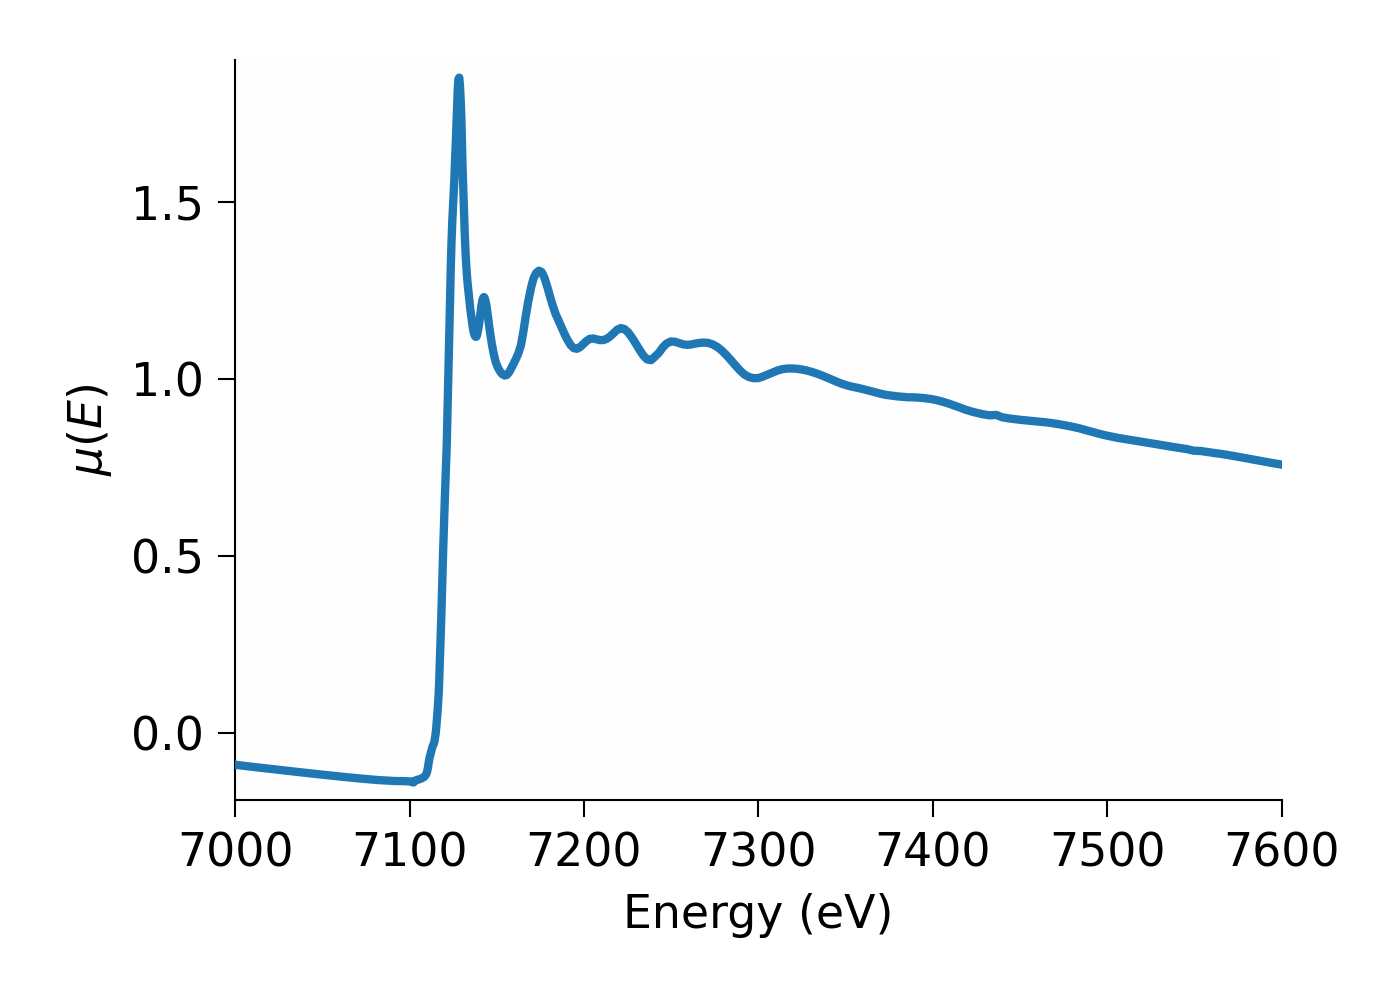
\includegraphics[width=35mm]{figs/experiment/feo_mu}

      \vmm
      Collected Spectra $\mu(E)$

    \end{column}
    \begin{column}{45mm}
      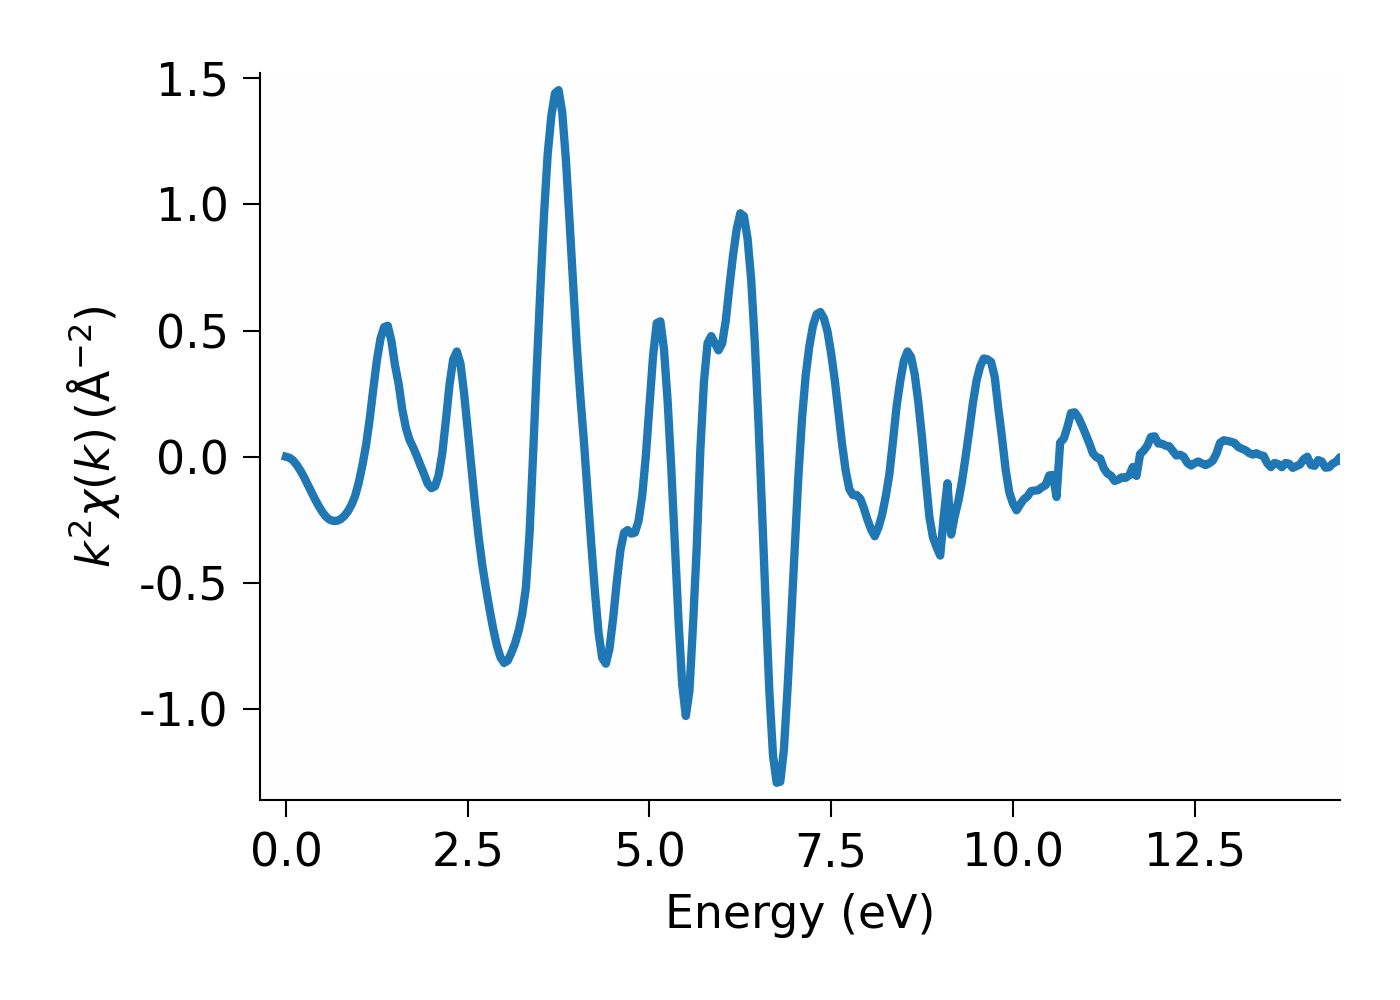
\includegraphics[width=35mm]{figs/experiment/feo_chik}

      \vmm
      Isolated $\chi(k)$, $k$-weighted

    \end{column}
    \begin{column}{45mm}
      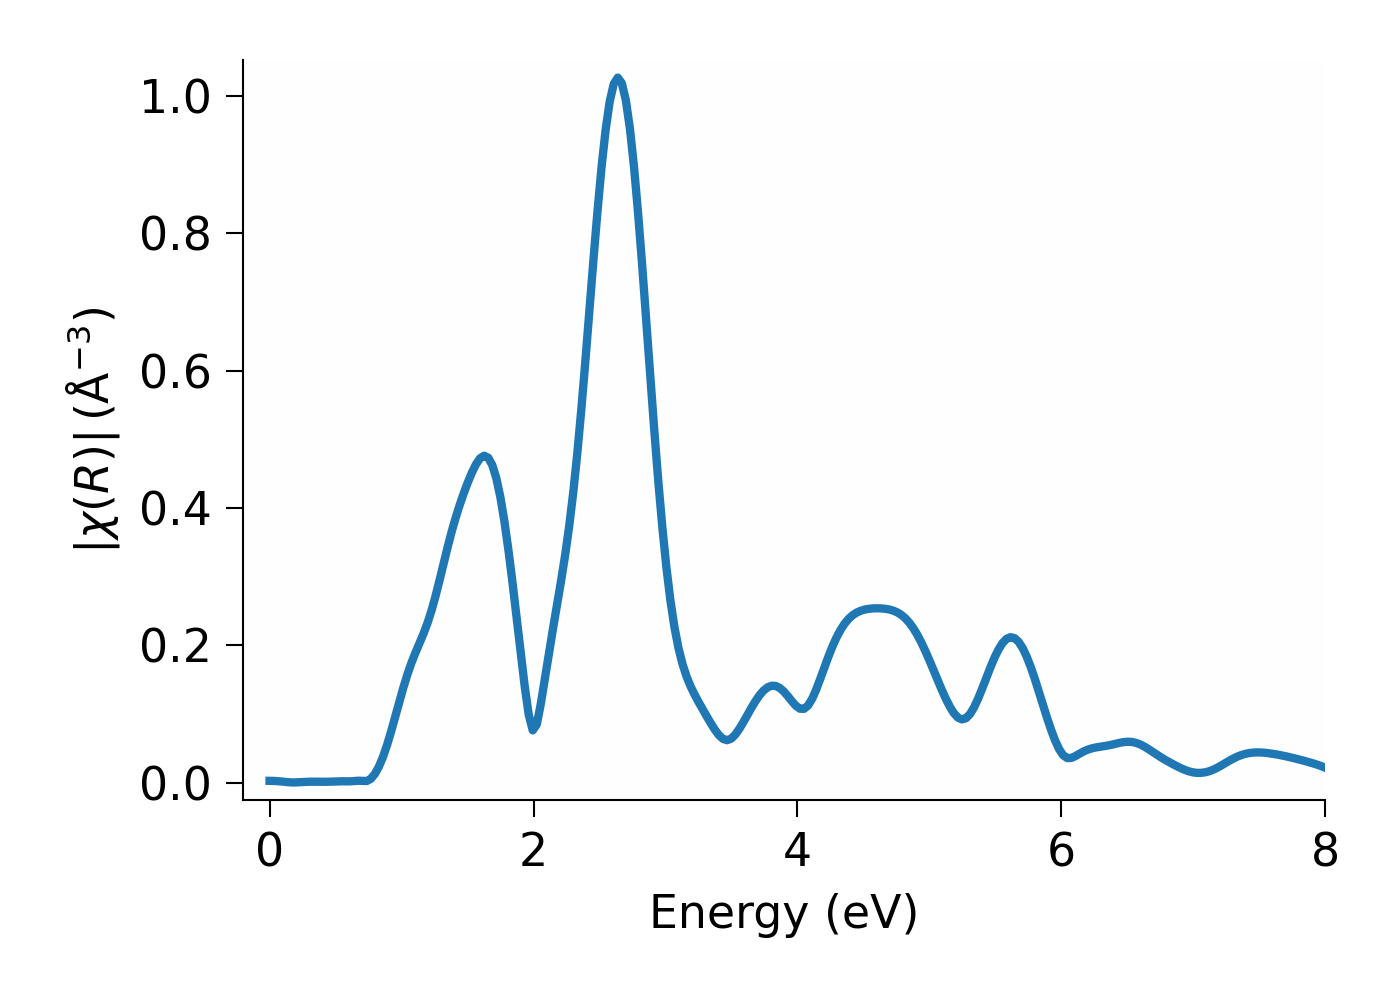
\includegraphics[width=35mm]{figs/experiment/feo_chir}

      \vmm
      $\chi(R)$, Fourier Transform of $\chi(k)$

    \end{column}
  \end{columns}

  \vmm \hrule

  \vmm\vmm

{\small{
  \begin{columns}[T]
    \begin{column}{65mm}
      \onslide+<2->

      Data Processing  features:
      \begin{itemize}
      \item  Data Visualization
      \item  Read in beamline data, merge data sets.
      \item  Pre-edge subtraction, Find $E_0$, Normalize Spectra
      \item  Background subtraction  to $\chi(k)$.
      \item  Fourier Transforms  $\chi(k) \rightarrow \chi(R)$.
      \item  Save/Read ``Projects'.
      \end{itemize}
    \vfill

  \end{column}

    \begin{column}{65mm}
   \onslide+<3->

   XANES Analysis features:
   \begin{itemize}
   \item  Pre-edge peak fitting.
   \item  Linear combination fits.
   \item Principal Component Analysis
   \end{itemize}

   Data Corrections:
   \begin{itemize}
   \item  Deglitching.
   \item  Energy Alignment.
   \item  Over-absorption Corrections.
   \item Smooth, Rebin, Deconvolutions.
   \end{itemize}

 \end{column}
\end{columns}

}}
\end{cenpage}


\end{slide}

\begin{slide}{ {\xasviewer} screenshots}

  \begin{cenpage}{145mm}

    \begin{columns}
    \begin{column}{75mm}
      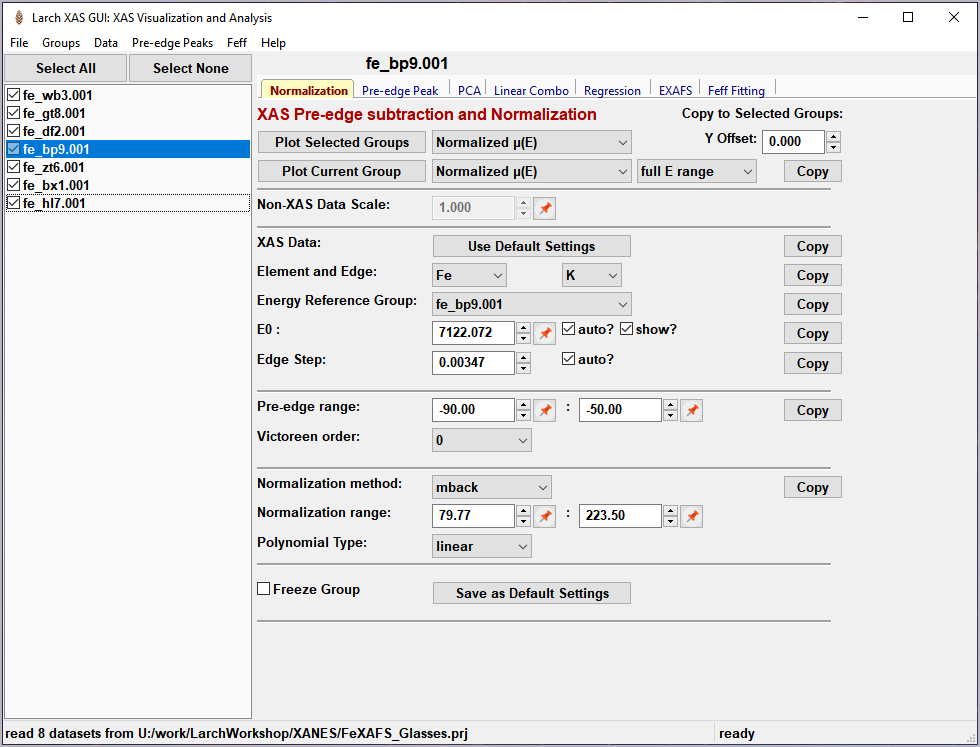
\includegraphics[width=75mm]{figs/Screenshots/XASViewer_Main}

      Panels for Normalization, Pre-edge Peak Fitting, PCA, Linear
      Combination Fitting, EXAFS (Background Subtraction+Fourier
      Transform), and Feff Fitting.

      \vfill
    \end{column}
    \begin{column}{30mm}
      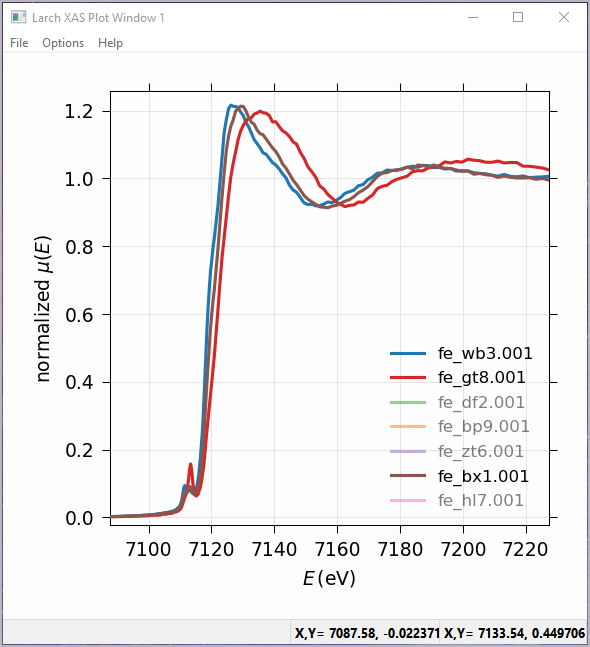
\includegraphics[width=30mm]{figs/Screenshots/XASViewer_MainPlot}

      \vmm
      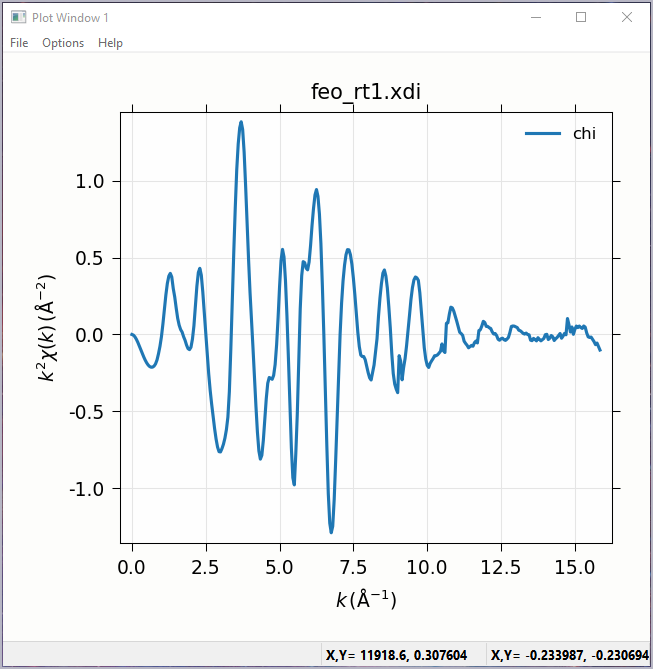
\includegraphics[width=30mm]{figs/Screenshots/XASViewer_EXAFS_plot1}

      \vmm \vfill
    \end{column}

      \begin{column}{30mm}
        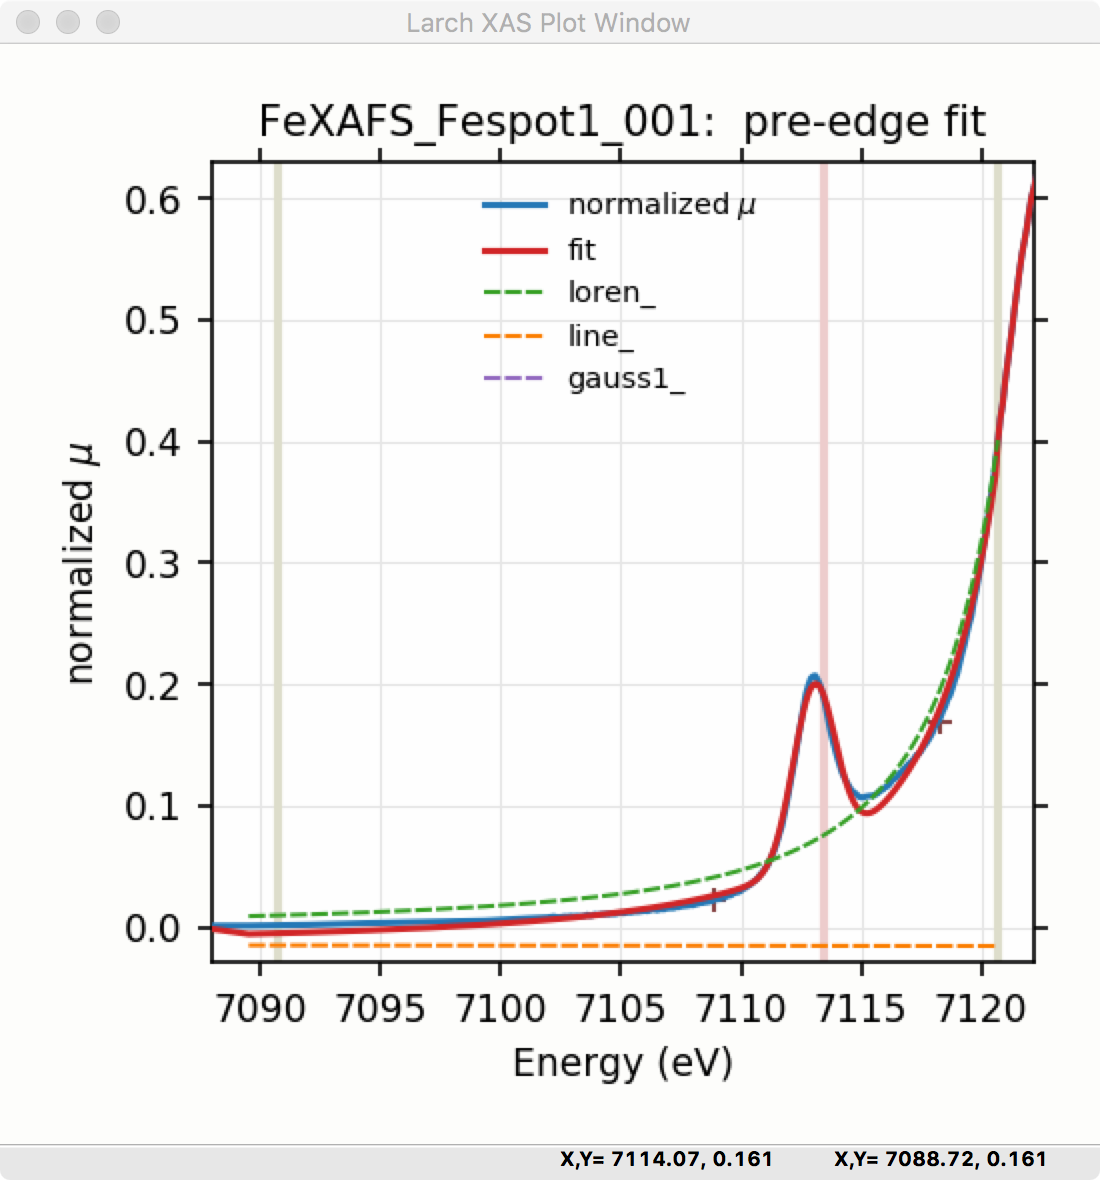
\includegraphics[width=30mm]{figs/Screenshots/XASViewer_plot_peakfit}

        \vmm
        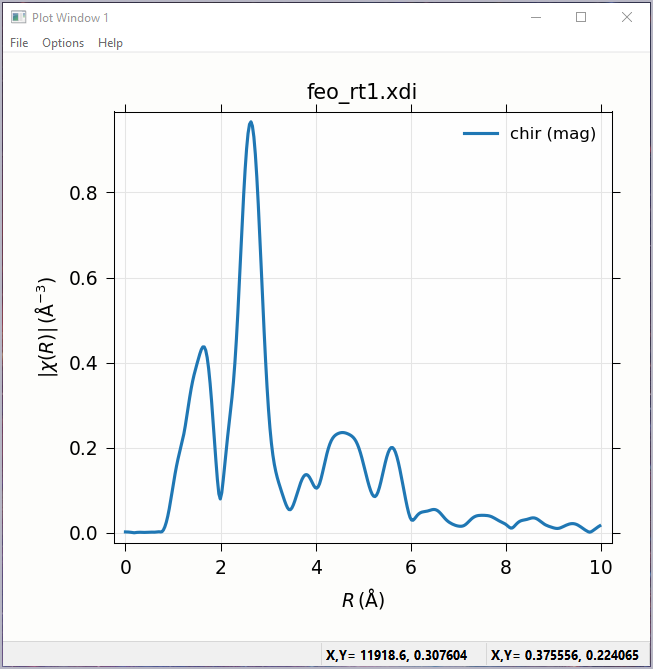
\includegraphics[width=30mm]{figs/Screenshots/XASViewer_EXAFS_plot_chir}

        \vmm \vfill
    \end{column}
\end{columns}

% \begin{tabular}{ll}
%   \begin{minipage}{75mm}  \wpdf{72mm}{figs/Athena_Screenshot} \end{minipage} &
%   \begin{minipage}{40mm}
%     \vspace{-3mm}   \wpdf{37mm}{figs/athena_mue}

%     \vspace{-3mm}   \wpdf{37mm}{figs/athena_chik}

%     \vspace{-3mm} \wpdf{37mm}{figs/athena_chir}
%   \end{minipage} \\
% \end{tabular}



 \end{cenpage}
\end{slide}


\section{Data Reduction Steps}

\begin{slide}{Data Reduction: Converting Raw Data to  {\mue}  }

  \begin{cenpage}{145mm}
    Step 1:   Starting with measured intensities,  we construct {\mue}:

    \vmm\vmm

    {    \only<1> {
    {\Blue{Transmission XAFS:}}   $ I_t = I_0 e^{-\mu(E)t)}  $  \hspace{10mm}  $ \mu(E)t =  - \ln(I_t/I_o)  $

    \vmm
    \begin{columns}
      \begin{column}{40mm}
        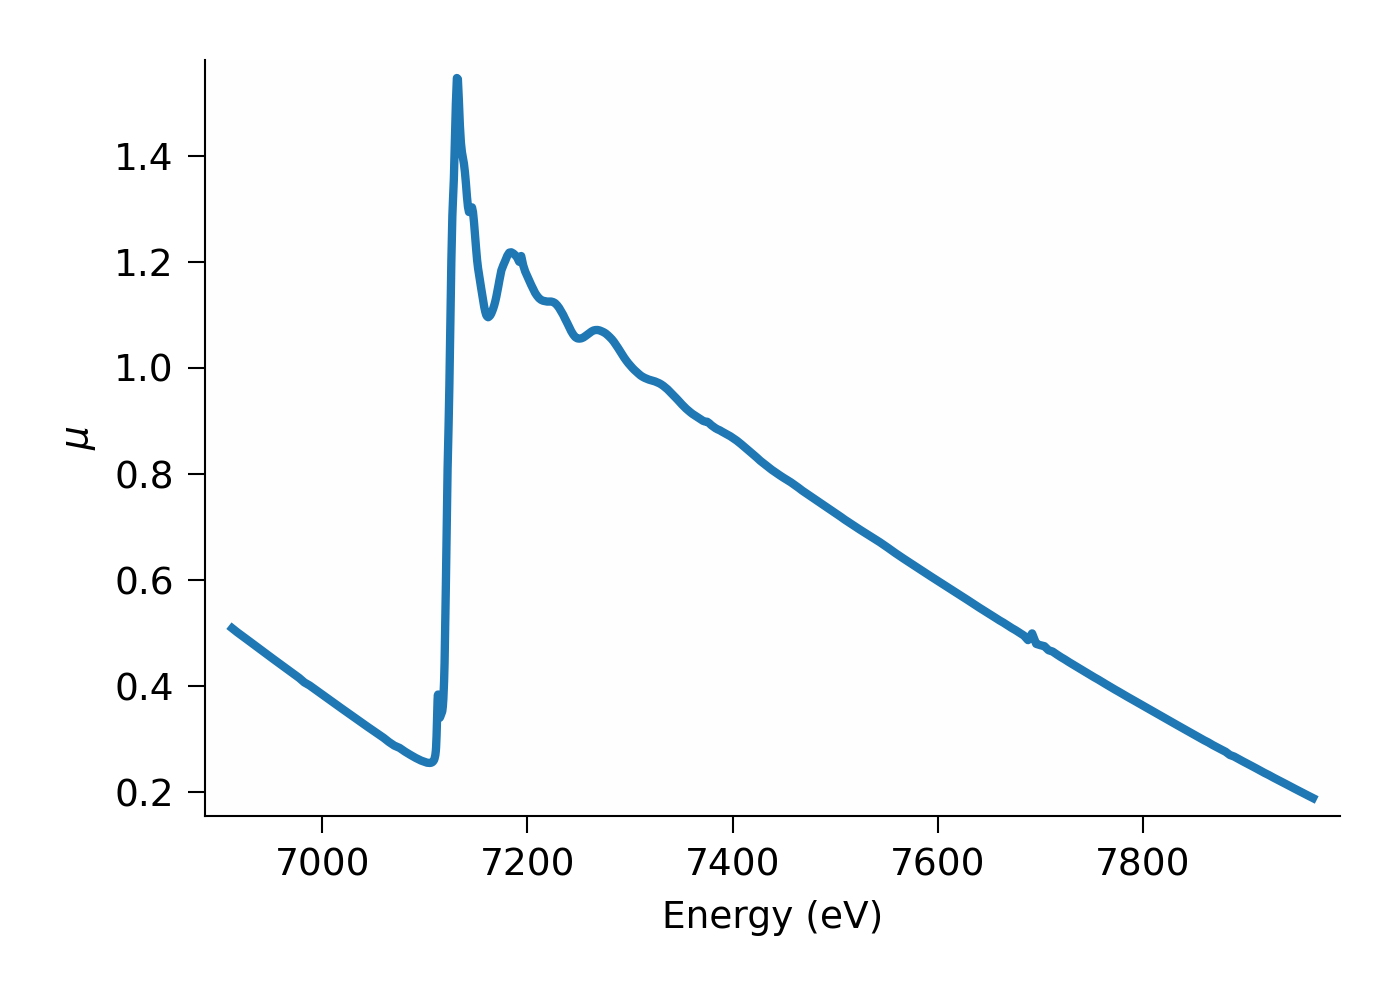
\includegraphics[width=40mm]{figs/experiment/mu}

        \hspace{15mm}        $\mu = -ln(I_t/I_0)$
      \end{column}
      \begin{column}{40mm}
        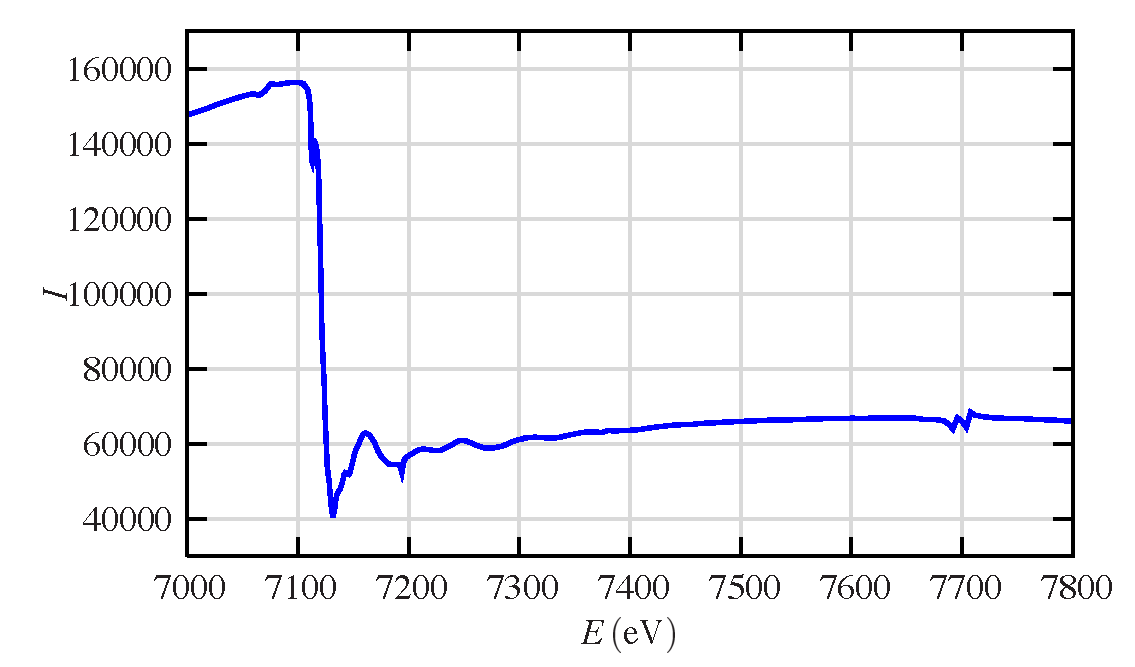
\includegraphics[width=40mm]{figs/experiment/i1}

        \hspace{15mm}        $I_t$
      \end{column}
      \begin{column}{40mm}
        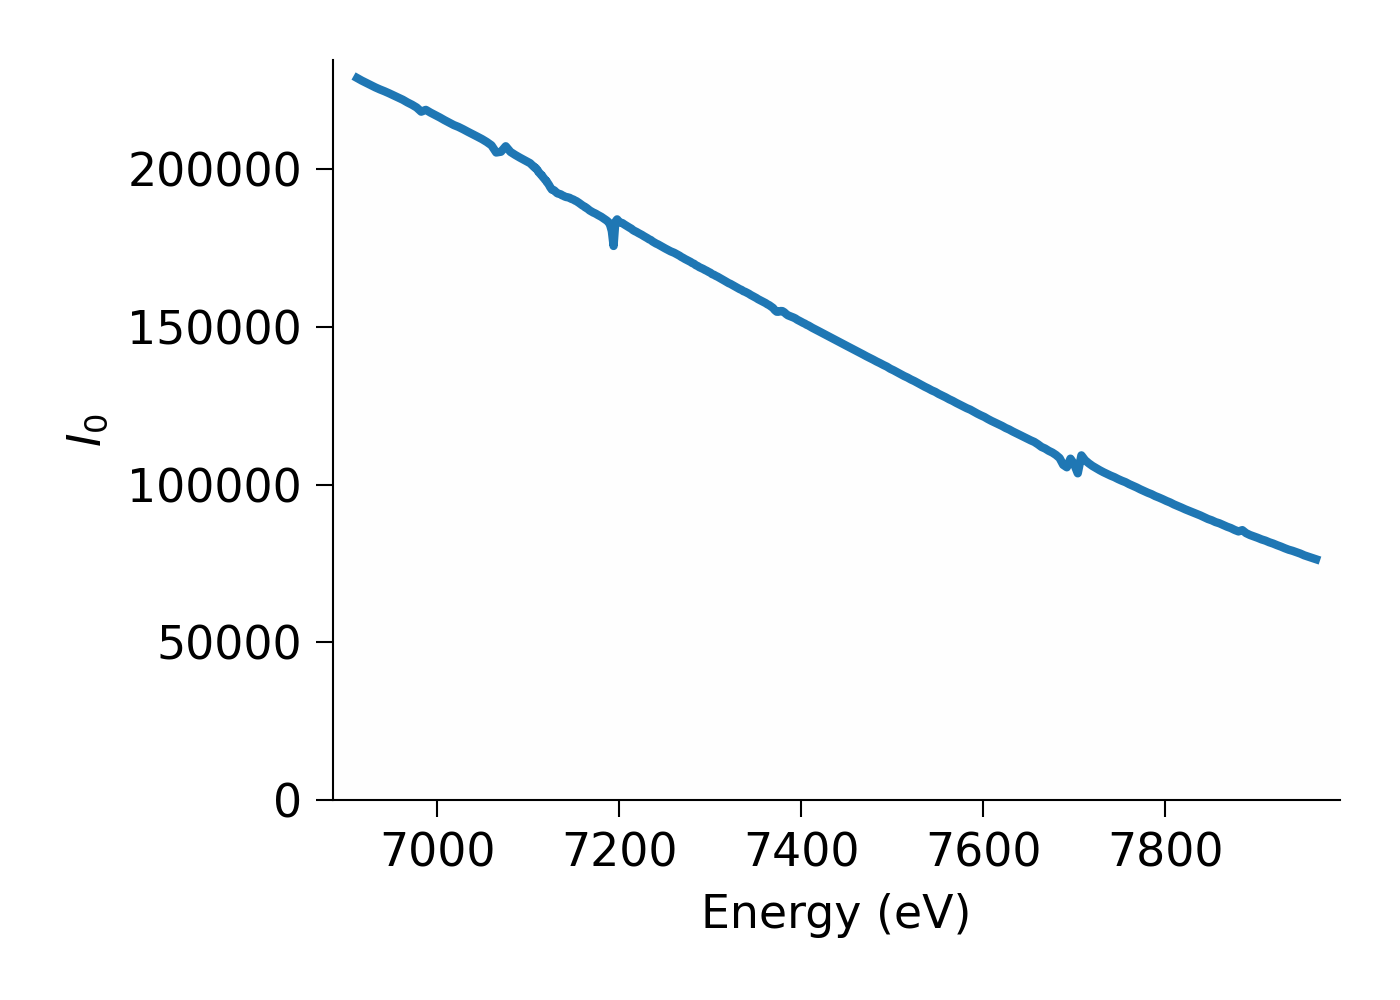
\includegraphics[width=40mm]{figs/experiment/i0}

        \hspace{15mm}        $I_0$
       \end{column}
     \end{columns}

     \vmm

  Transmission measurements are needed for high concentration elements, above
  ($\sim 5 {\rm wt \%}$).



   }}

 {\only<2> {

    {\Blue{Fluorescence XAFS:}}   $ \mu(E) \propto I_f / I_0 $

    \vmm
    \begin{columns}
      \begin{column}{40mm}
        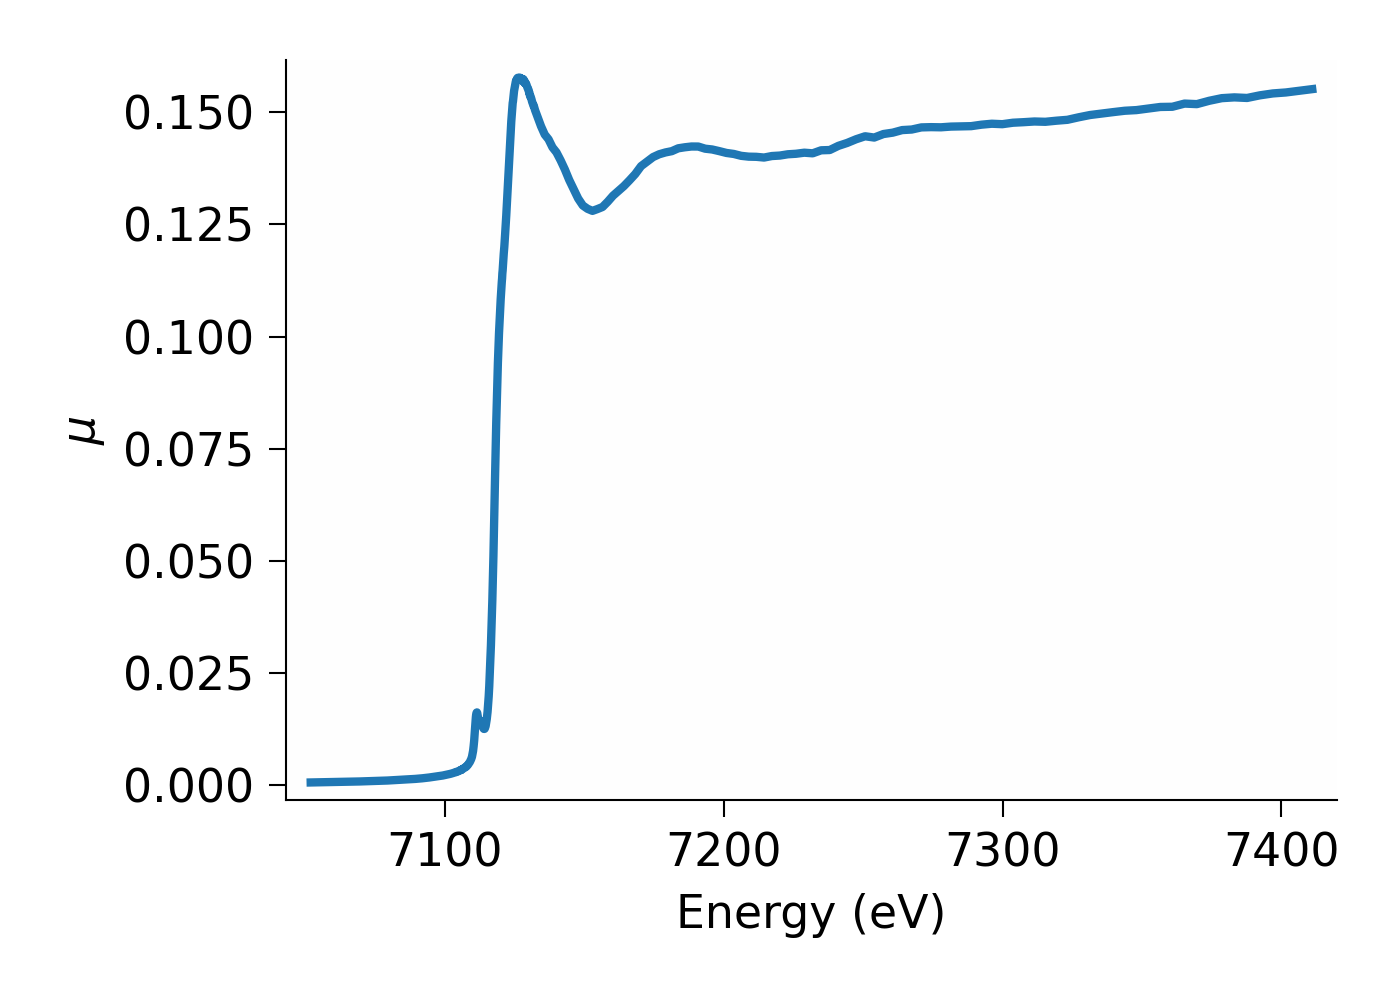
\includegraphics[width=40mm]{figs/experiment/mu_fluor}

        \hspace{15mm}        $\mu = (I_f/I_0)$
      \end{column}
      \begin{column}{40mm}
        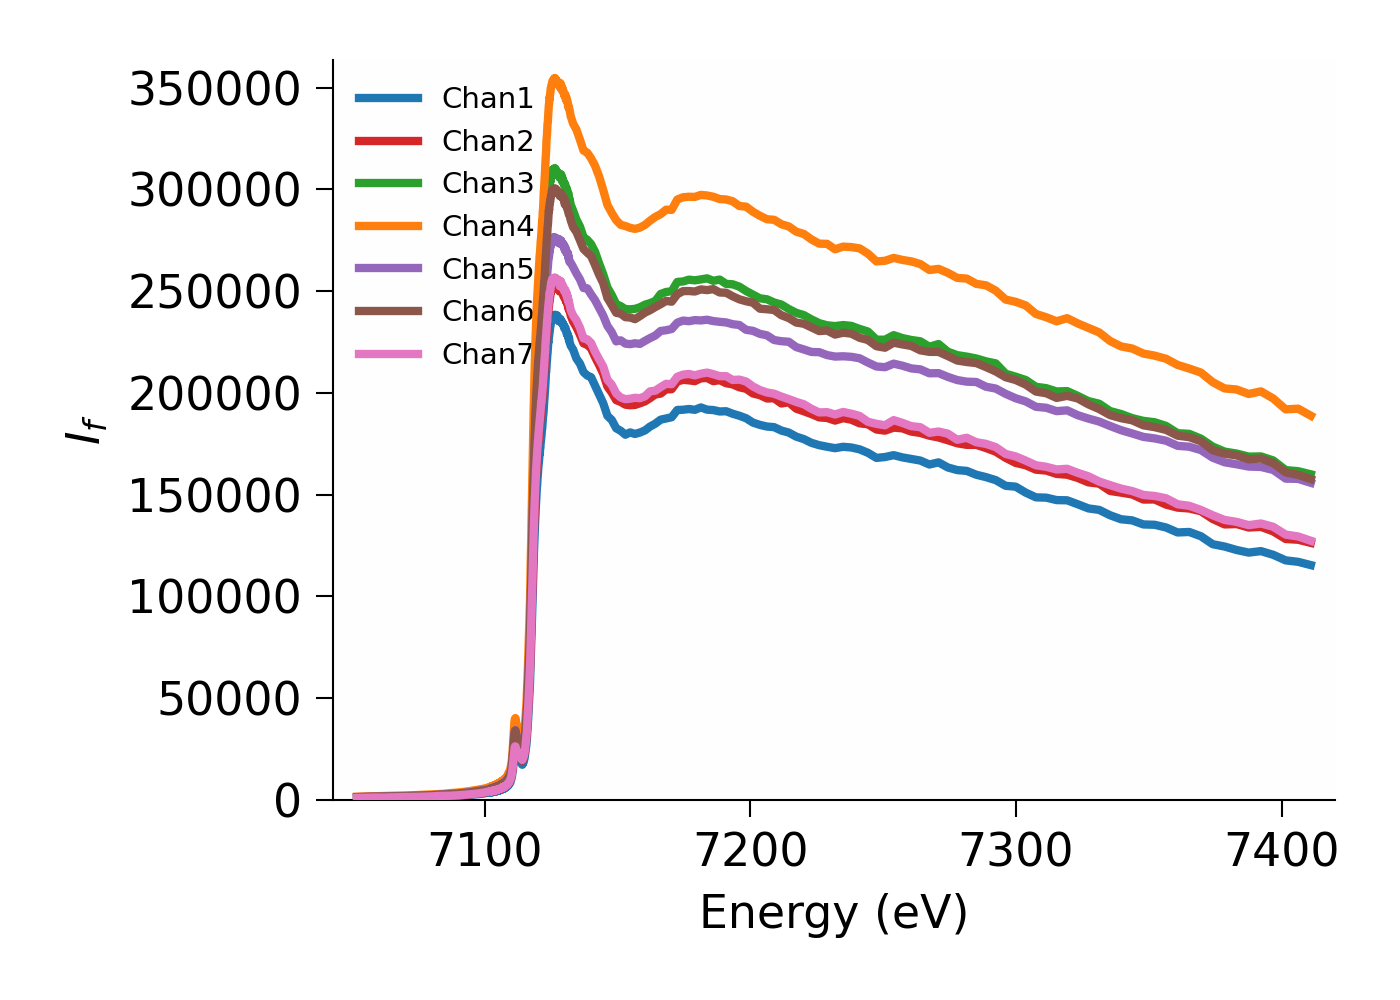
\includegraphics[width=40mm]{figs/experiment/if_multi}

        \hspace{15mm}        $I_f$
      \end{column}
      \begin{column}{40mm}
        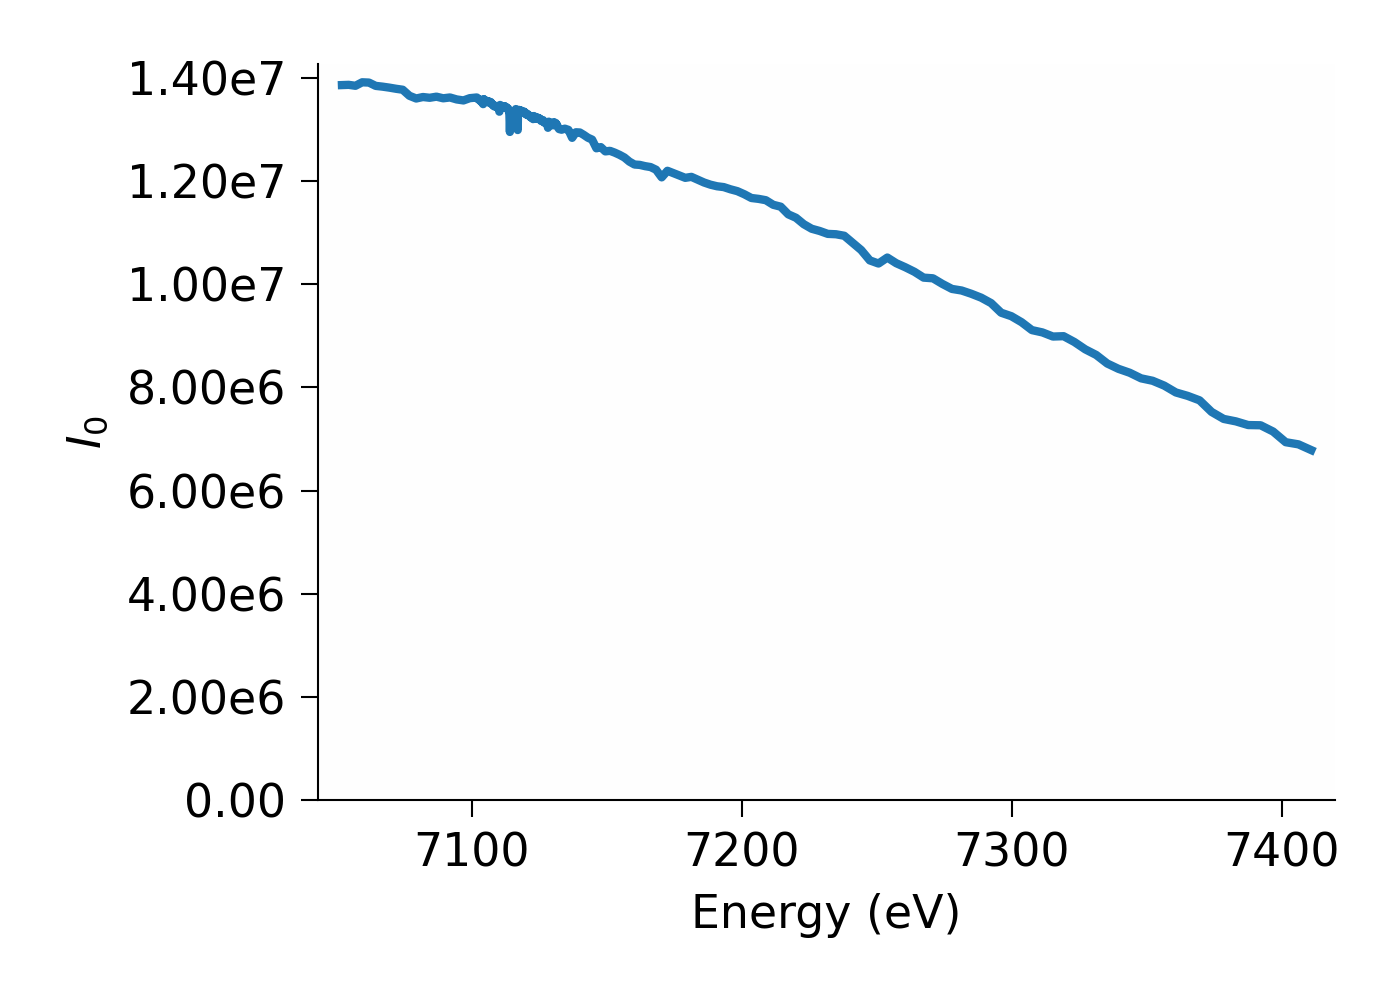
\includegraphics[width=40mm]{figs/experiment/i0_fluor}

        \hspace{15mm}        $I_0$
       \end{column}
     \end{columns}

 \vmm\vmm


 here $I_f$ may be:

 \begin{itemize}
 \item  the intensity from a single fluorescence ion chamber (Lytle detector).
 \item  the {\RedEmph{sum}} of several signals from a multi-element solid-state detector.
 \item  other emission measurement (electron yield, visible light)
 \end{itemize}

 \vmm


 Fluorescence measurements are generally better for
 elements at concentrations below  ($\sim 5 {\rm wt  \%}$).

}}

  \vfill

\end{cenpage}
\end{slide}

\begin{slide}{Merging Data, Aligning Data, Deglitching }

Real Data is typically measured in several scans.  These scans can be
{\BlueEmph{merged}} together to give better statistics.

\vmm
Important issues when processing data

\begin{cenpage}{120mm}
\begin{itemize}
\item The monochromator energy calibration may drift with time.
  \begin{itemize}
    \item scans can be aligned so that $E_0$ is constant for all scans.
    \item a {\BlueEmph{Reference Channel}} -- often a metal foil -- can be
      measured {\RedEmph{during the scan}} and used for energy alignment.
    \item if the drift is bad enough (every scan, etc), consult the
      beamline scientist.
  \end{itemize}
\item At certain energies, $I_0$ jumps -- a {\BlueEmph{glitch}} -- that may
  not normalize out of {\mue}.  These points should be removed.
\item {\RedEmph{over-absorption}} for concentrated samples measured in
  fluorescence.
  \end{itemize}
\end{cenpage}

{\xasviewer}  can help with these. So can {\athena} and {\sixpack}.



\end{slide}

\begin{frame} \frametitle{Data Reduction: Pre-Edge Subtraction, Normalization}

  \begin{cenpage}{130mm}

    \begin{tabular}{ll}
      \begin{minipage}{70mm} 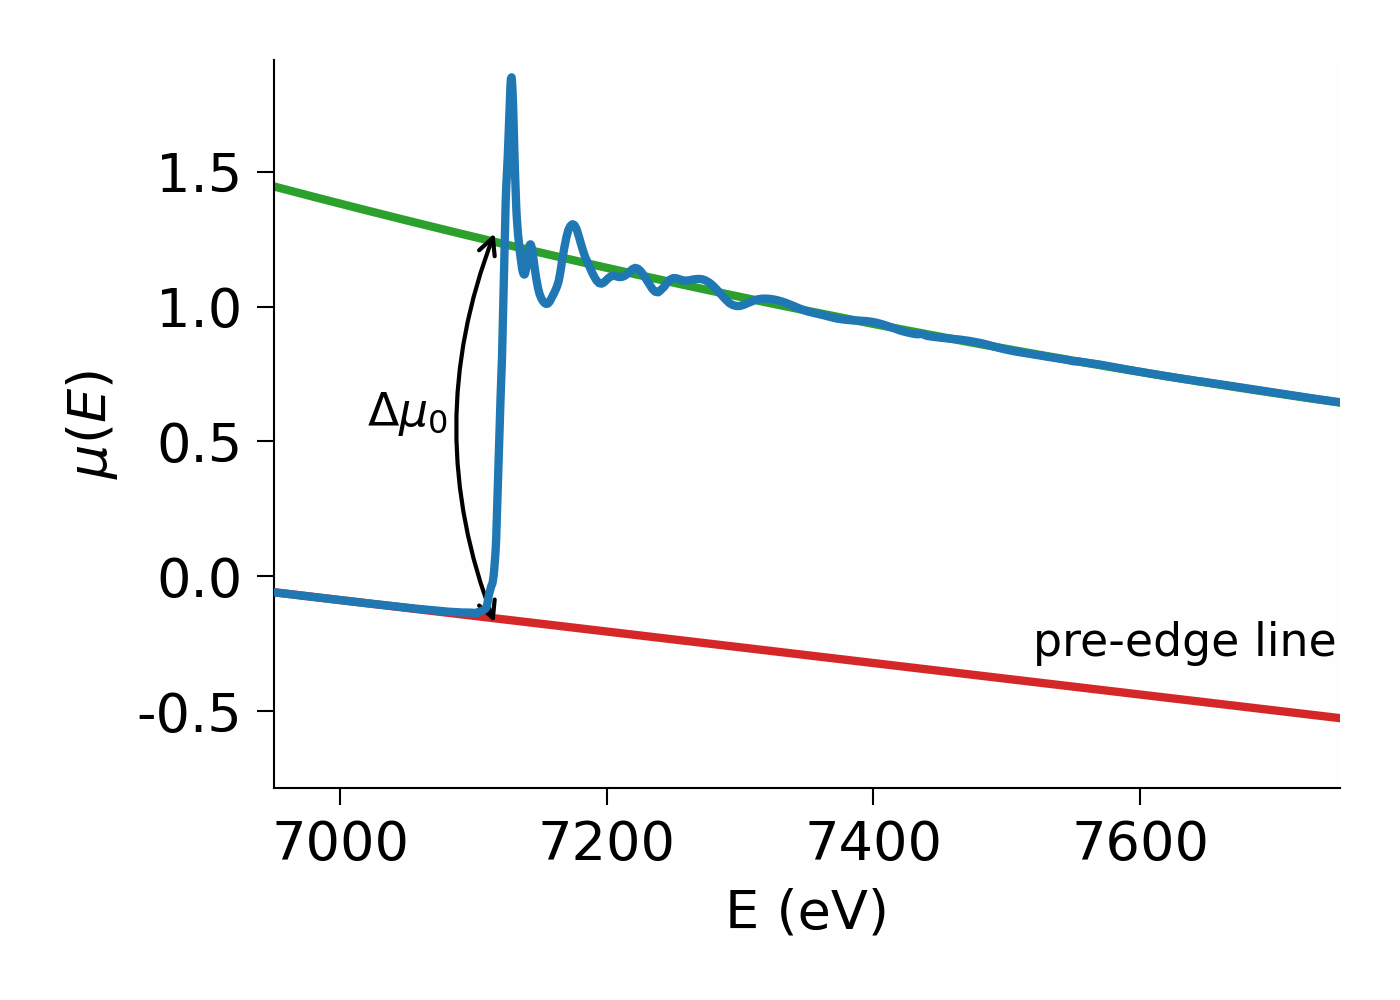
\includegraphics[width=60mm]{figs/experiment/mu_preedge}   \end{minipage}
      &
      \begin{minipage}{45mm}
        \setlength{\baselineskip}{10pt}
        \hspace{-3mm}{\Red{Pre-Edge Subtraction}}\vspace{0.5mm}

        We subtract away the background that fits the {\RedEmph{pre-edge}}
        region.  This gets rid of the absorption due to other absorption
        edges   (say, the  Fe ${\rm L_{\rm III}}$ edge).

     \end{minipage}\\
      \begin{minipage}{70mm} 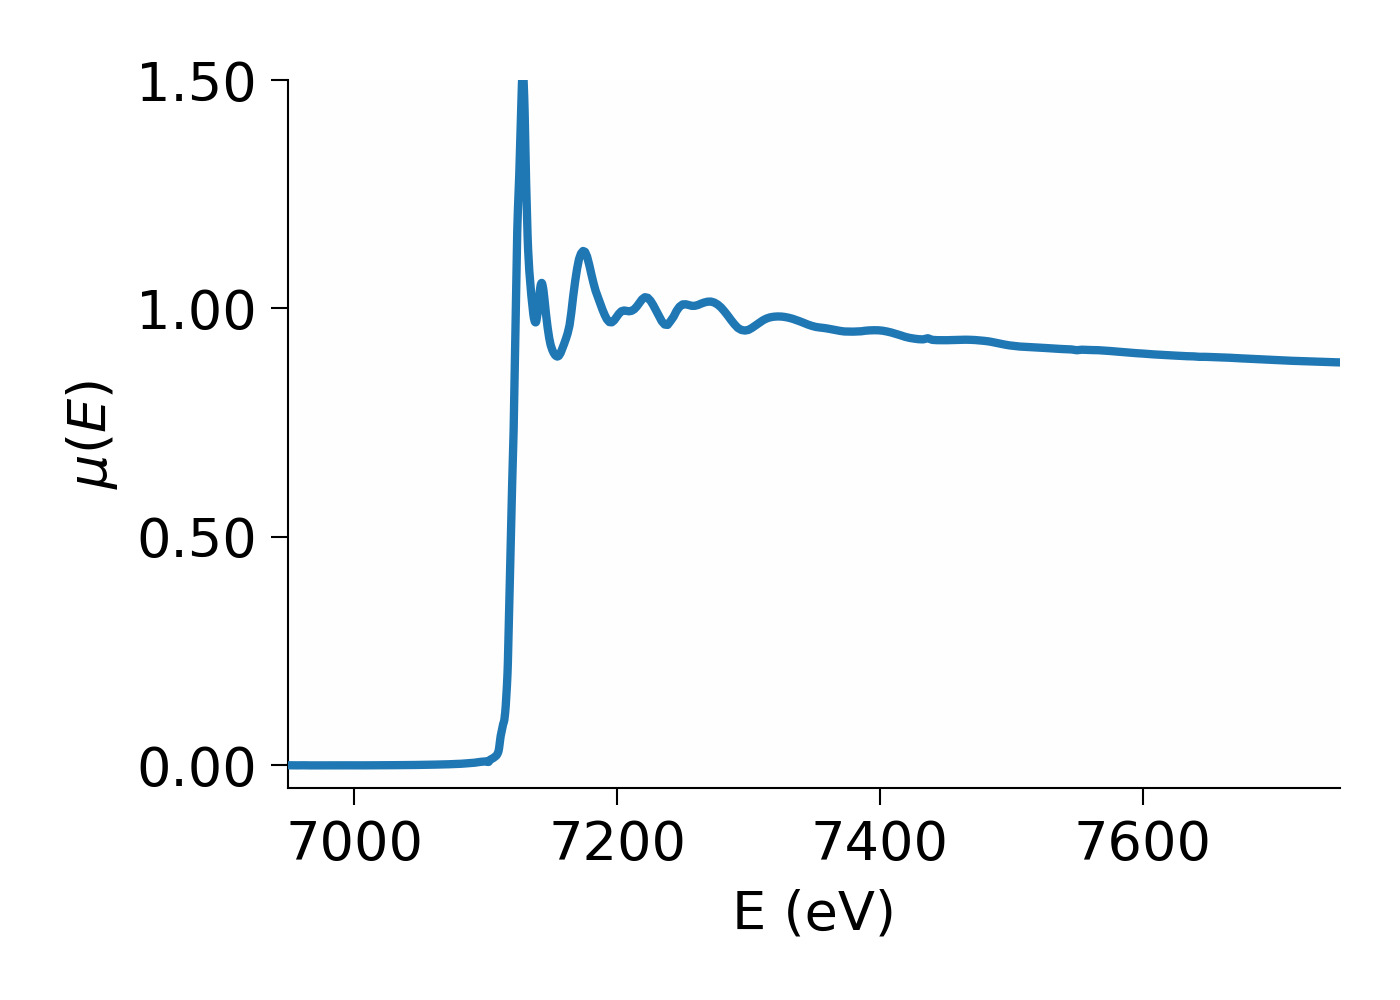
\includegraphics[width=60mm]{figs/experiment/mu_norm}  \end{minipage}
      &
      \begin{minipage}{45mm} \setlength{\baselineskip}{10pt}
        \hspace{-3mm}{\Red{Normalization}}\vspace{0.5mm}


        We estimate the {\RedEmph{edge step}}, ${\Delta \mu_0(E_0)}$
        by extrapolating a simple curve the above {\mue} to the
        edge.
        \[ \mu_{\rm norm}(E) = \mu(E) /  {\Delta \mu_0(E_0)} \]

        \vmm

      \end{minipage}
    \end{tabular}
    \end{cenpage}
\end{frame}

\begin{frame}\frametitle{Data Reduction: Normalized XANES and ${E_0}$}

  \begin{cenpage}{130mm}

  \begin{tabular}{ll}
    \begin{minipage}{70mm}  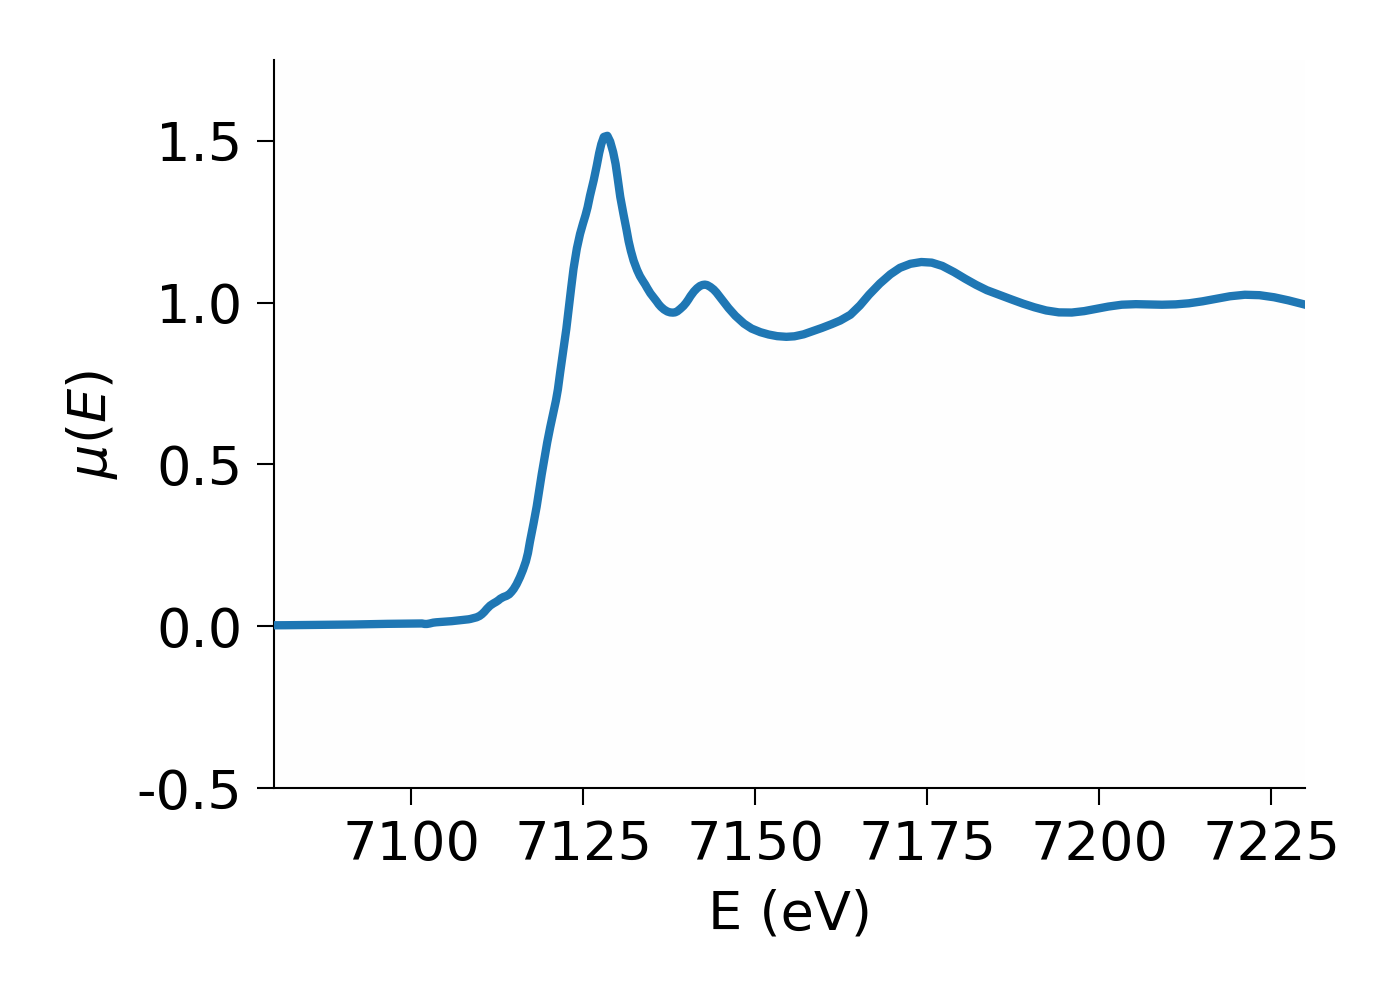
\includegraphics[width=60mm]{figs/experiment/mu_norm_xanes}  \end{minipage}
    &
    \begin{minipage}{45mm}  \setlength{\baselineskip}{10pt}
      \hspace{-3mm}{\Red{XANES}}\vspace{0.5mm}

      The XANES part of {\mue} shows a fairly rich spectral structure.
      We'll use $\mu_{\rm norm}(E)$  for XANES analysis.

    \end{minipage}\\
    \begin{minipage}{70mm} 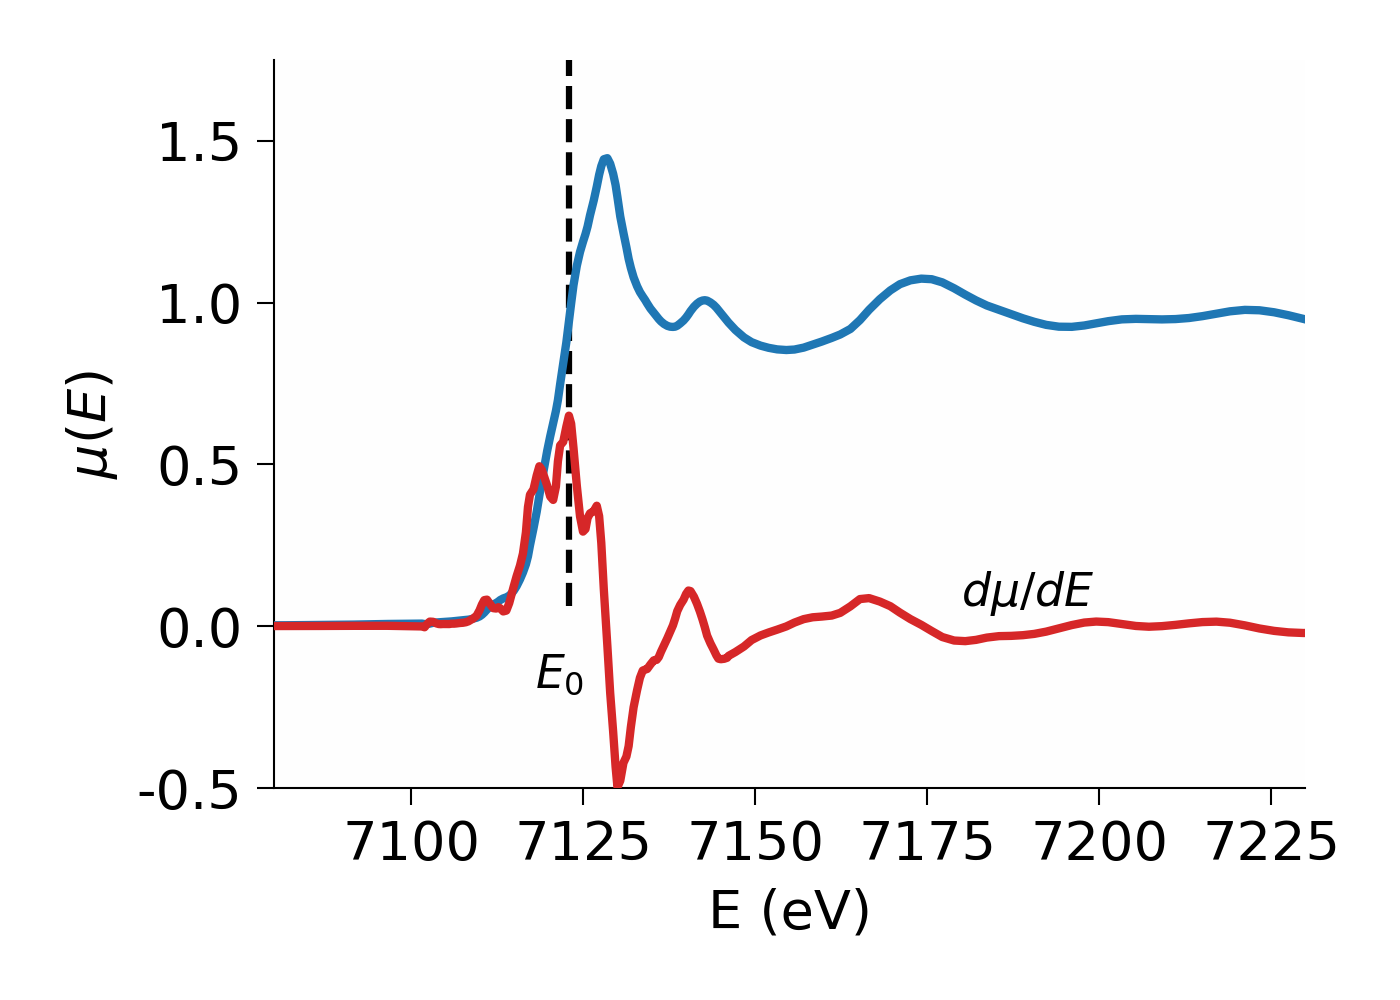
\includegraphics[width=60mm]{figs/experiment/mu_xanes_deriv}  \end{minipage}
    &
    \begin{minipage}{45mm}  \setlength{\baselineskip}{10pt}
      \hspace{-3mm}{\Red{Derivative}}\vspace{0.5mm}

      We can select ${E_0}$ roughly as the energy with the maximum
      derivative.  This is somewhat arbitrary, so we'll keep in mind that
      we may need to refine this value later on.
    \end{minipage}
  \end{tabular}
    \end{cenpage}
\end{frame}


\begin{frame}\frametitle{Data Reduction: Normalization with tabulated $\mu(E)$}

  \begin{cenpage}{130mm}

  \begin{tabular}{ll}
    \begin{minipage}{70mm}  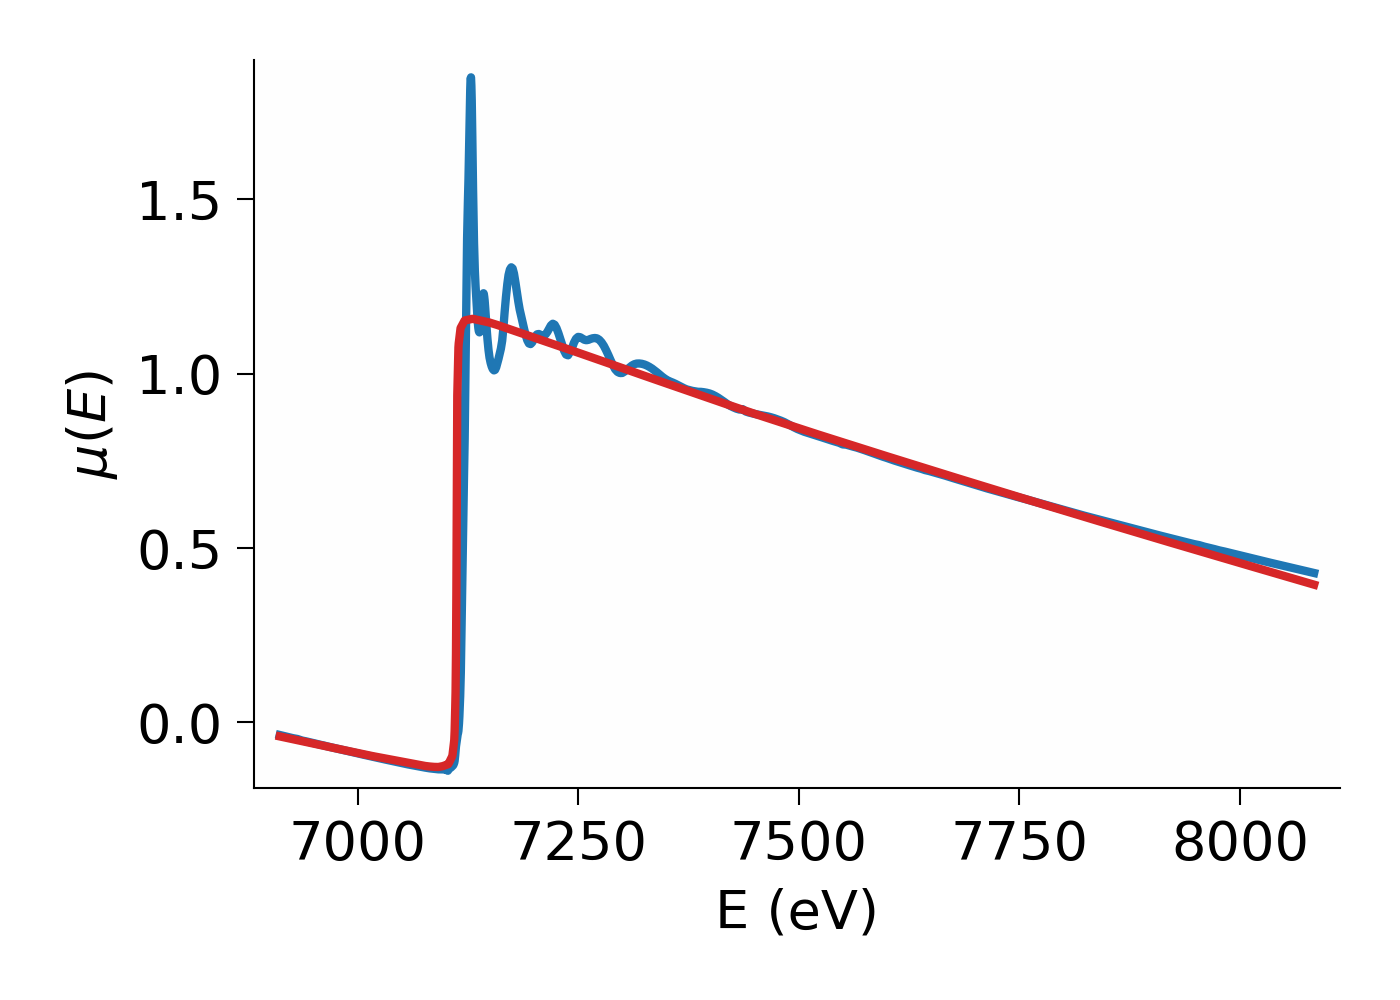
\includegraphics[width=60mm]{figs/experiment/mu_mback}  \end{minipage}
    &
    \begin{minipage}{45mm}  \setlength{\baselineskip}{10pt}
      \hspace{-3mm}{\Red{Using tabulated $\mu(E)$ }}\vspace{0.5mm}

      Tabulated values (Chanter, et al) can also be used to normalize the
      data.

      \vmm
      This can improve consistency, as the same functional fom is
      used for all spectra of an element and edge.

    \end{minipage}\\
    \begin{minipage}{70mm} 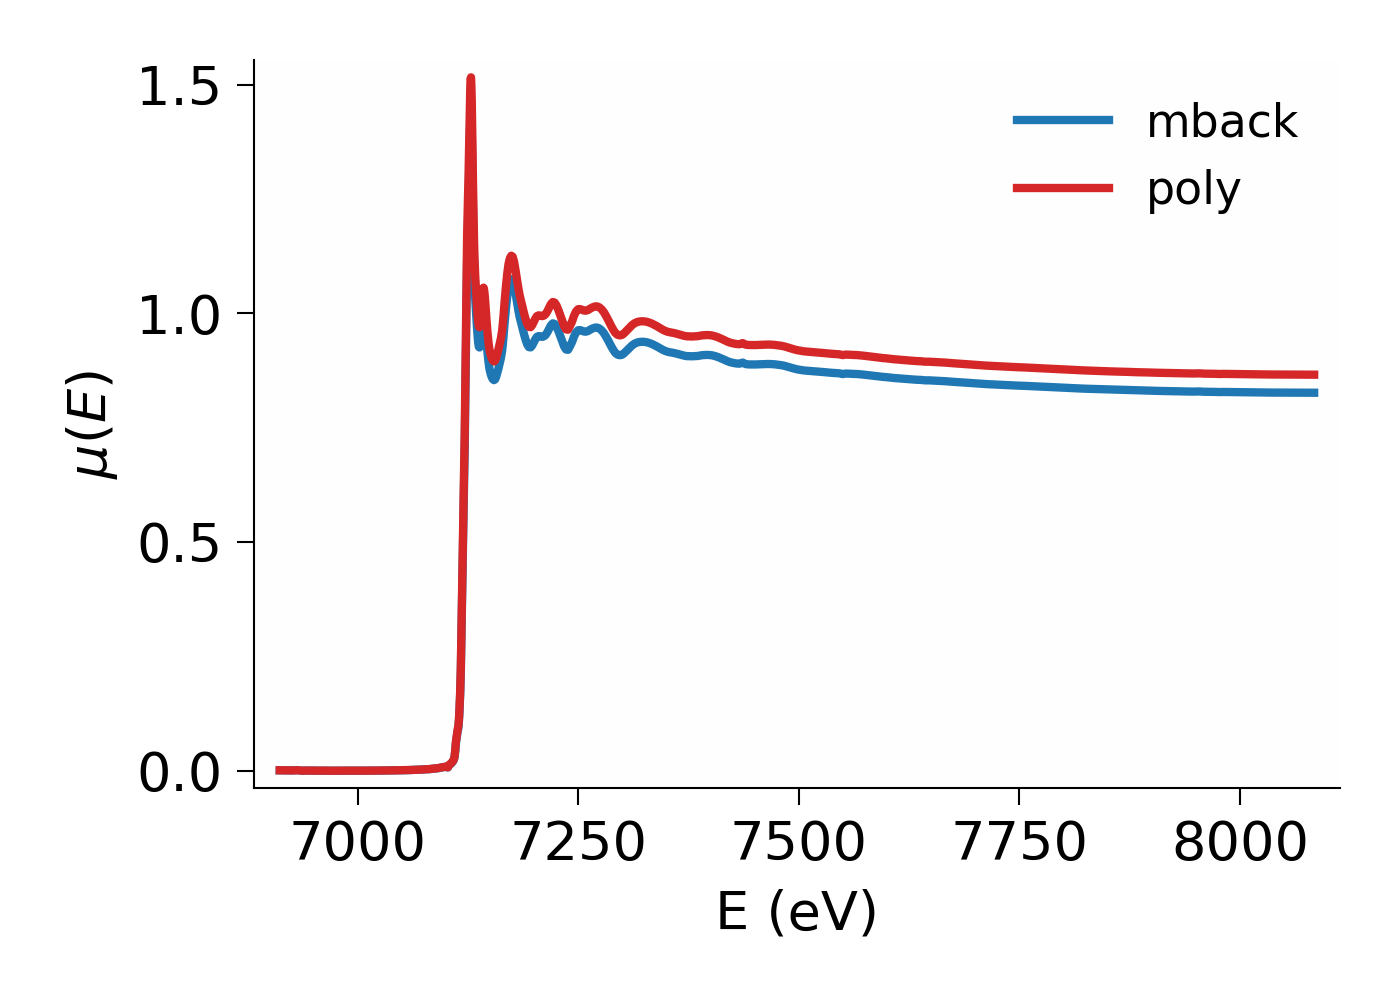
\includegraphics[width=60mm]{figs/experiment/mu_mback_poly}  \end{minipage}
    &
    \begin{minipage}{45mm}  \setlength{\baselineskip}{10pt}
      \hspace{-3mm}{\Red{Polynomial vs tabulated values}}\vspace{0.5mm}

      The difference is typically at the margin, but consistency is good!

      \vmm
      This is based on the {\mback} procedure of T.C. Weng, et al.

    \end{minipage}
  \end{tabular}
    \end{cenpage}
\end{frame}


\begin{frame} \frametitle{Data Reduction: Post-Edge Background Subtraction}

    \begin{cenpage}{130mm}

  \begin{tabular}{ll}
    \begin{minipage}{70mm} 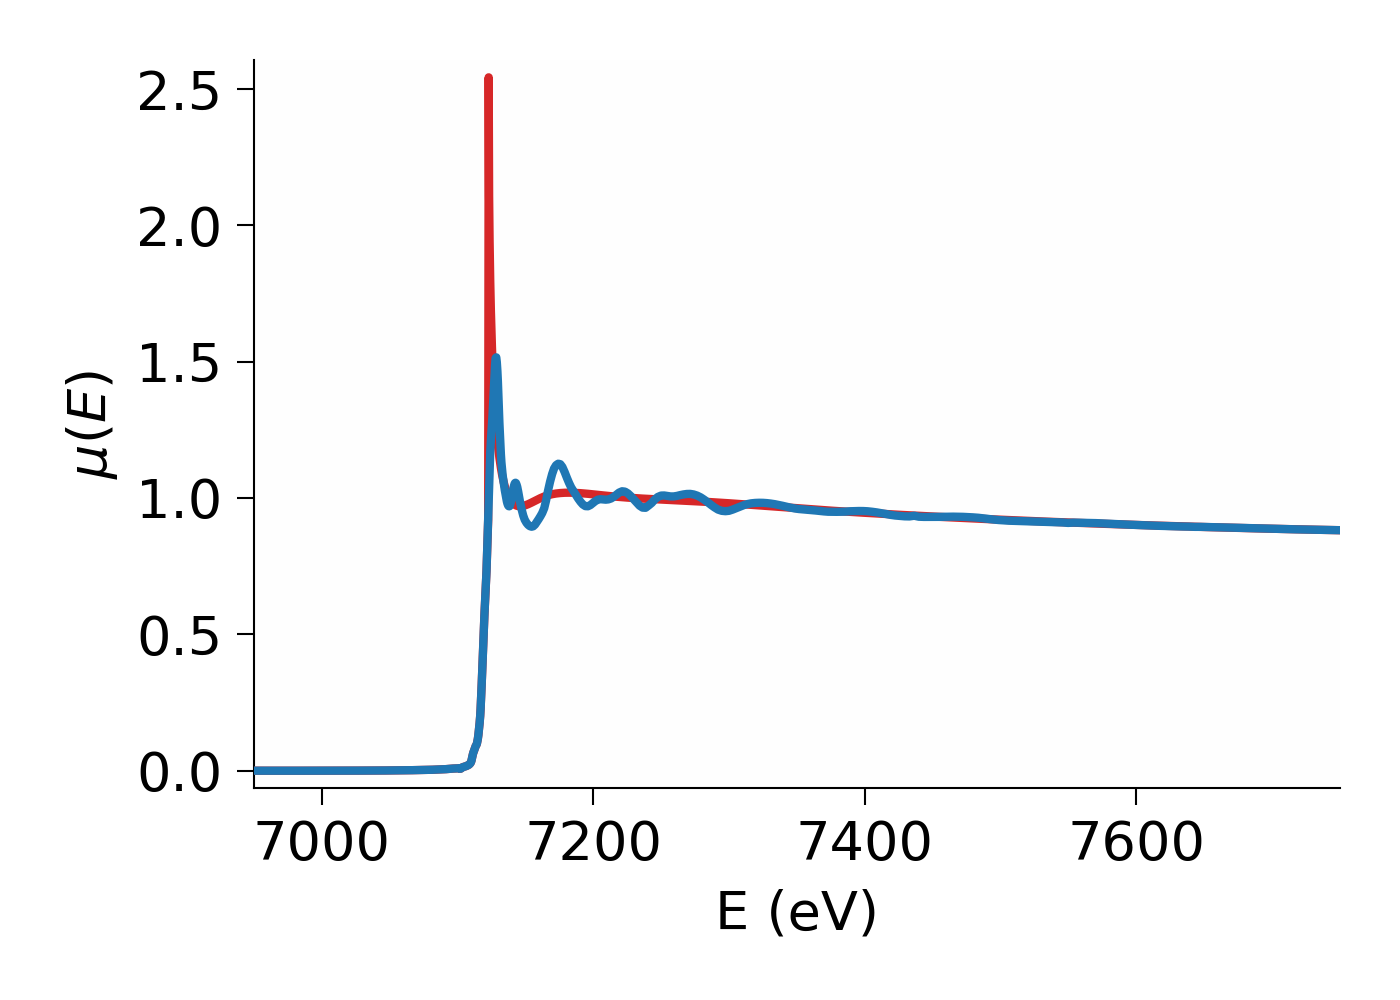
\includegraphics[width=60mm]{figs/experiment/bkg_full}  \end{minipage}
    &
    \begin{minipage}{50mm}  \setlength{\baselineskip}{10pt}
      \hspace{-3mm}{\Red{Post-Edge Background}}\vspace{0.5mm}

      \[ \chi(E) = \frac{\mu(E) -\mu_0(E)}{\Delta \mu_0(E_0)} \]

      We don't have a measurement of {\bkg} (the absorption
      coefficient without neighboring atoms).

      \vspace{1mm}

    \end{minipage}\\
    \begin{minipage}{70mm} 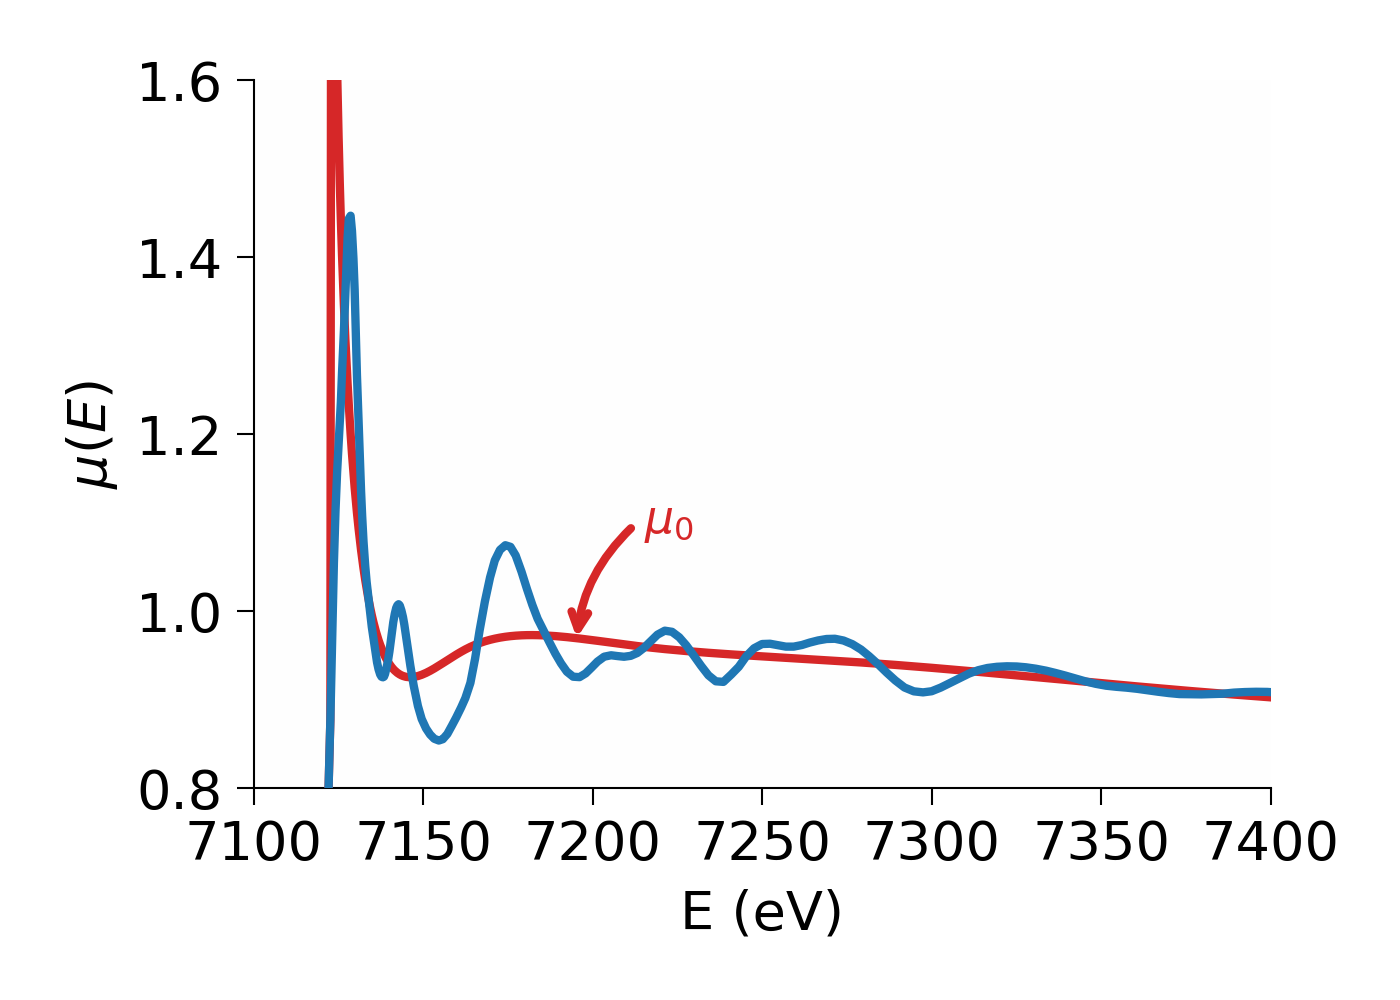
\includegraphics[width=60mm]{figs/experiment/bkg_xanes}  \end{minipage}
    &
    \begin{minipage}{50mm} \setlength{\baselineskip}{10pt}

      We approximate {\bkg} by an adjustable, smooth
      function: a {\BlueEmph{spline}}.

      \vmm

      This can be dangerous -- a flexible enough
      spline could match {\mue} and remove all the EXAFS!
      We want a spline that will match the {\BlueEmph{low frequency}}
      components of {\mue}.

    \end{minipage}
  \end{tabular}
    \end{cenpage}

\end{frame}


\begin{frame} \frametitle{Data Reduction: {\chie} to {\chik}}

  \begin{cenpage}{130mm}

    \begin{tabular}{ll}
    \begin{minipage}{70mm} 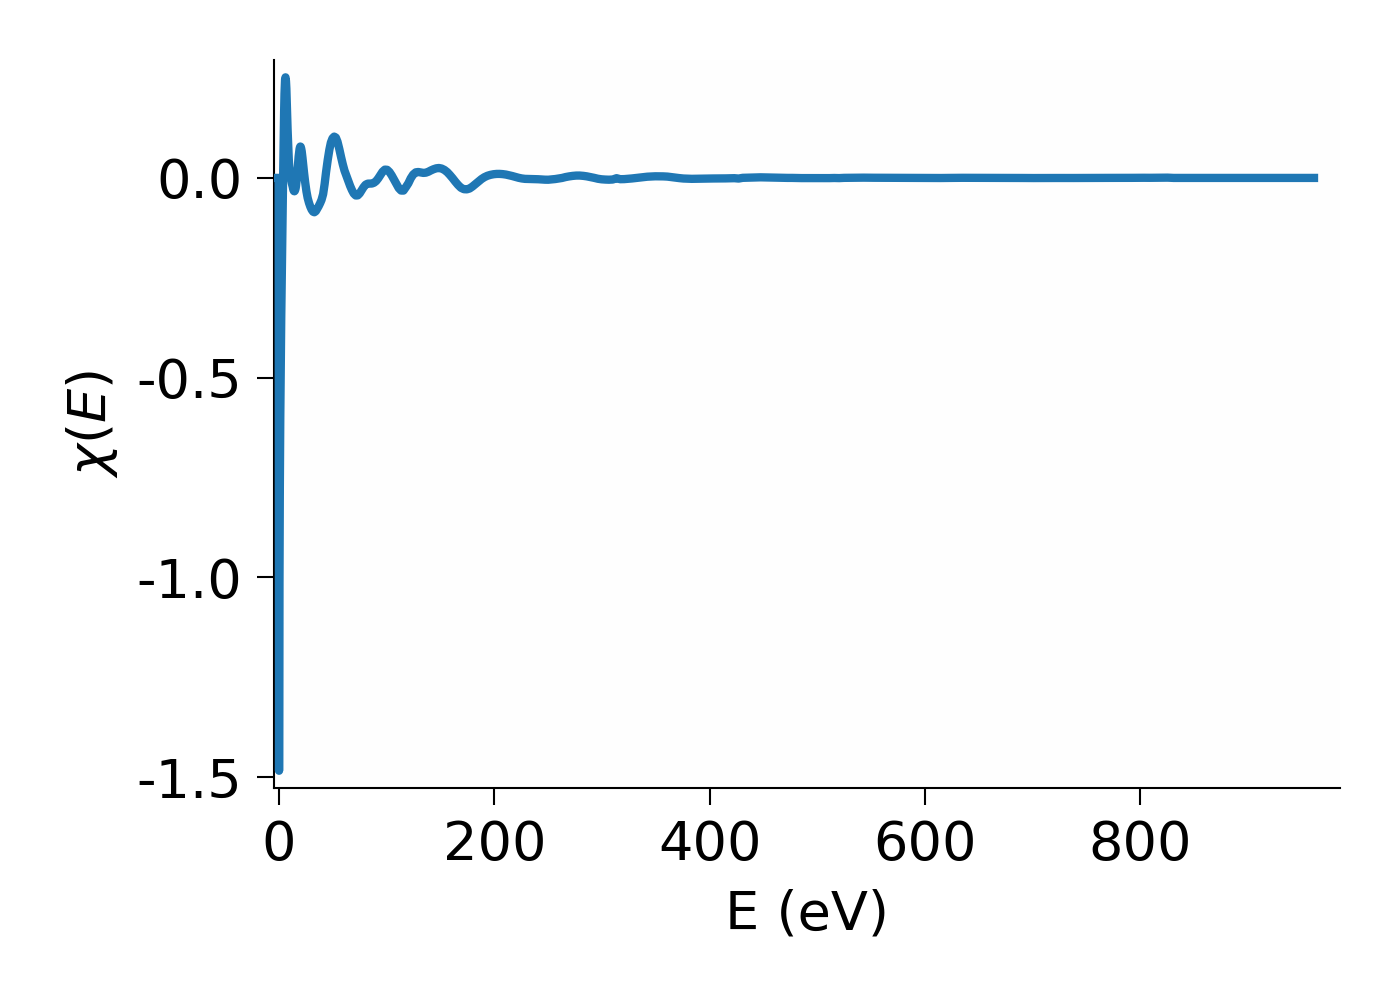
\includegraphics[width=60mm]{figs/experiment/chie}  \end{minipage}
    &
    \begin{minipage}{45mm}  \setlength{\baselineskip}{10pt}
      \hspace{-3mm}{\Red{$ \chi(E)$ }}\vmm

      \[ \chi(E) = \frac{\mu(E) -\mu_0(E)}{\Delta \mu_0(E_0)} \]

      where $ \Delta \mu_0(E_0) $ is the Edge Step found earlier.

      \vfill
    \end{minipage}\\
    \begin{minipage}{70mm} 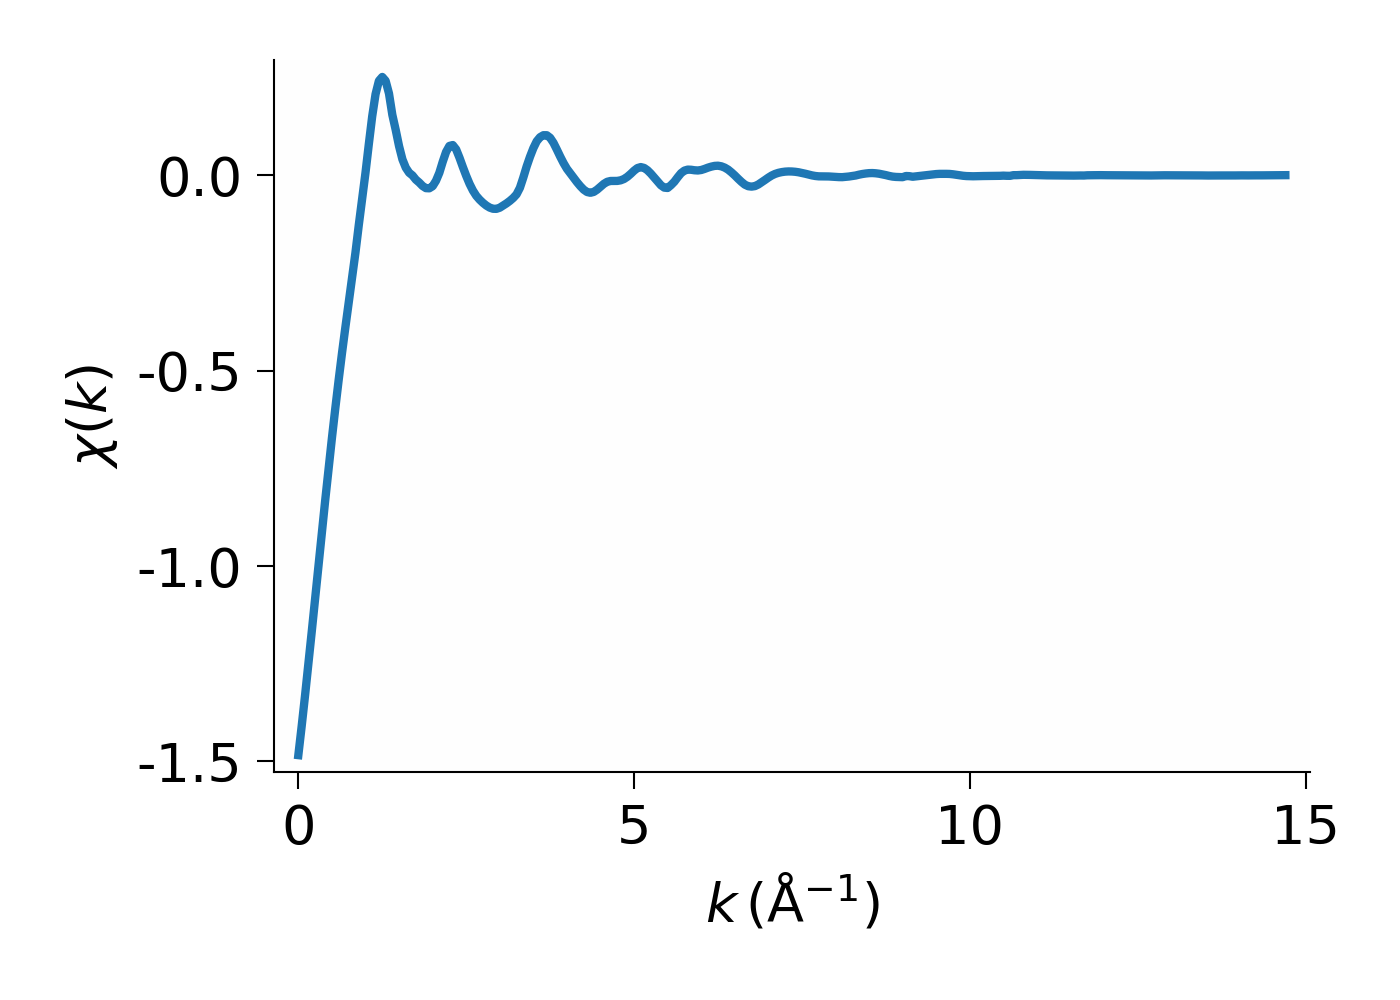
\includegraphics[width=60mm]{figs/experiment/chik}  \end{minipage}
    &
    \begin{minipage}{45mm} \setlength{\baselineskip}{10pt}
      \hspace{-3mm}{\Red{$\chi(k)$}}       \vmm

      Convert scale from Energy, $E$, to wavenumber $k$:

       \[ k= \sqrt{{{2m(E-E_0)}\over{\hbar^2}}} \]

      \vfill
    \end{minipage}
  \end{tabular}
\end{cenpage}

\end{frame}

\begin{frame} \frametitle{Data Reduction: {\chik}, ${k}$-weighting}

  \begin{cenpage}{130mm}
  \begin{tabular}{ll}
    \begin{minipage}{70mm} 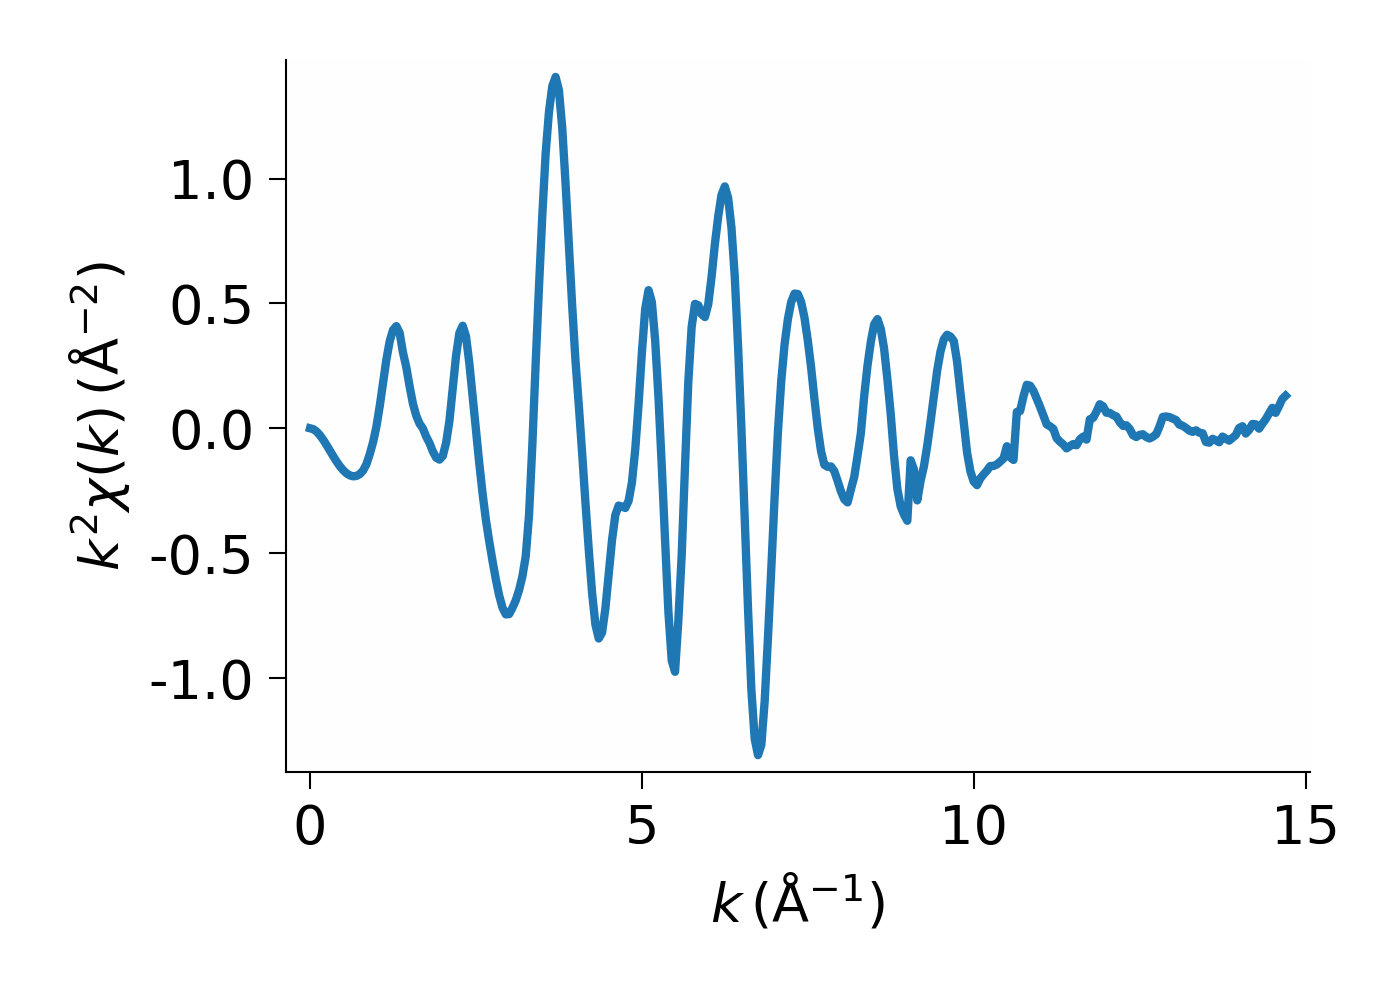
\includegraphics[width=60mm]{figs/experiment/chikw}  \end{minipage}
    &
    \begin{minipage}{45mm}  \setlength{\baselineskip}{10pt}
      \hspace{-3mm}{\Red{\chik}}\vmm

      The raw EXAFS {\chik} decays quickly with $k$.

      \vmm

      We emphasize the higher-$k$ portion of the spectra by
      multiplying by  ${k^2}$ or ${k^3}$.
      \vfill
    \end{minipage}\\
    \begin{minipage}{70mm}
      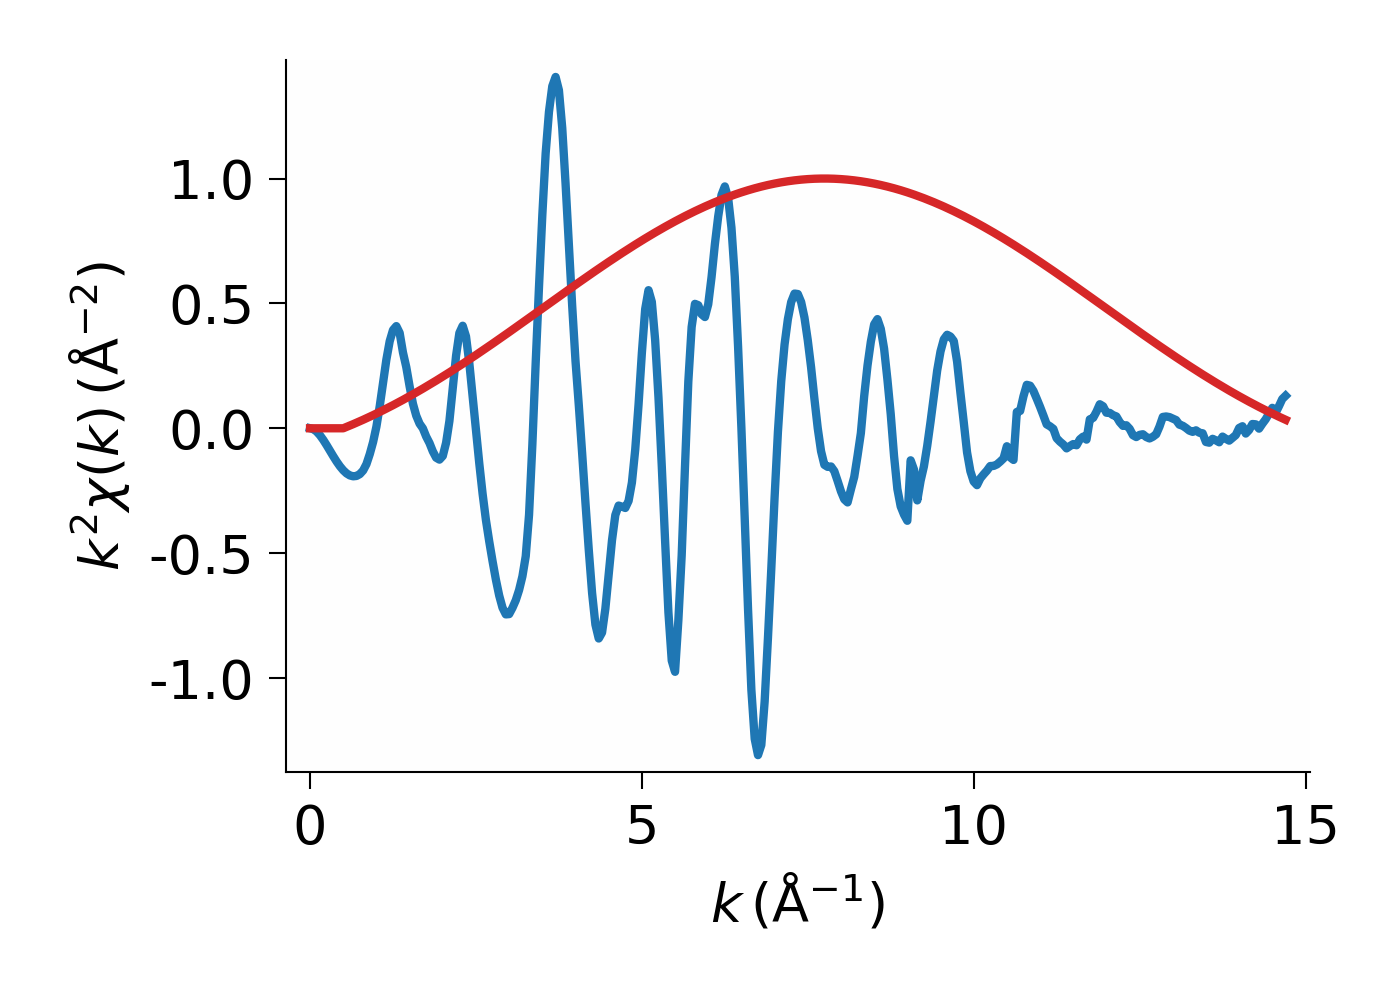
\includegraphics[width=60mm]{figs/experiment/chikw_win}  \end{minipage}
    &
    \begin{minipage}{45mm} \setlength{\baselineskip}{10pt}
      \hspace{-3mm}{\Red{$k$-weighted $\chi(k)$:
          ${k^2\chi(k)}$}}\vspace{0.5mm}

      {\chik} is composed of sine waves, so we'll Fourier Transform from
      $k$ to $R$-space.

      \vmm To avoid ``ringing'', we'll multiply by a
      {\BlueEmph{window function}}.  \vfill
    \end{minipage}
  \end{tabular}
\end{cenpage}

\end{frame}

\begin{frame} \frametitle{EXAFS Fourier Transform: ${\chi(R)}$}

  \begin{cenpage}{130mm}
    \begin{tabular}{ll}
    \begin{minipage}{70mm} 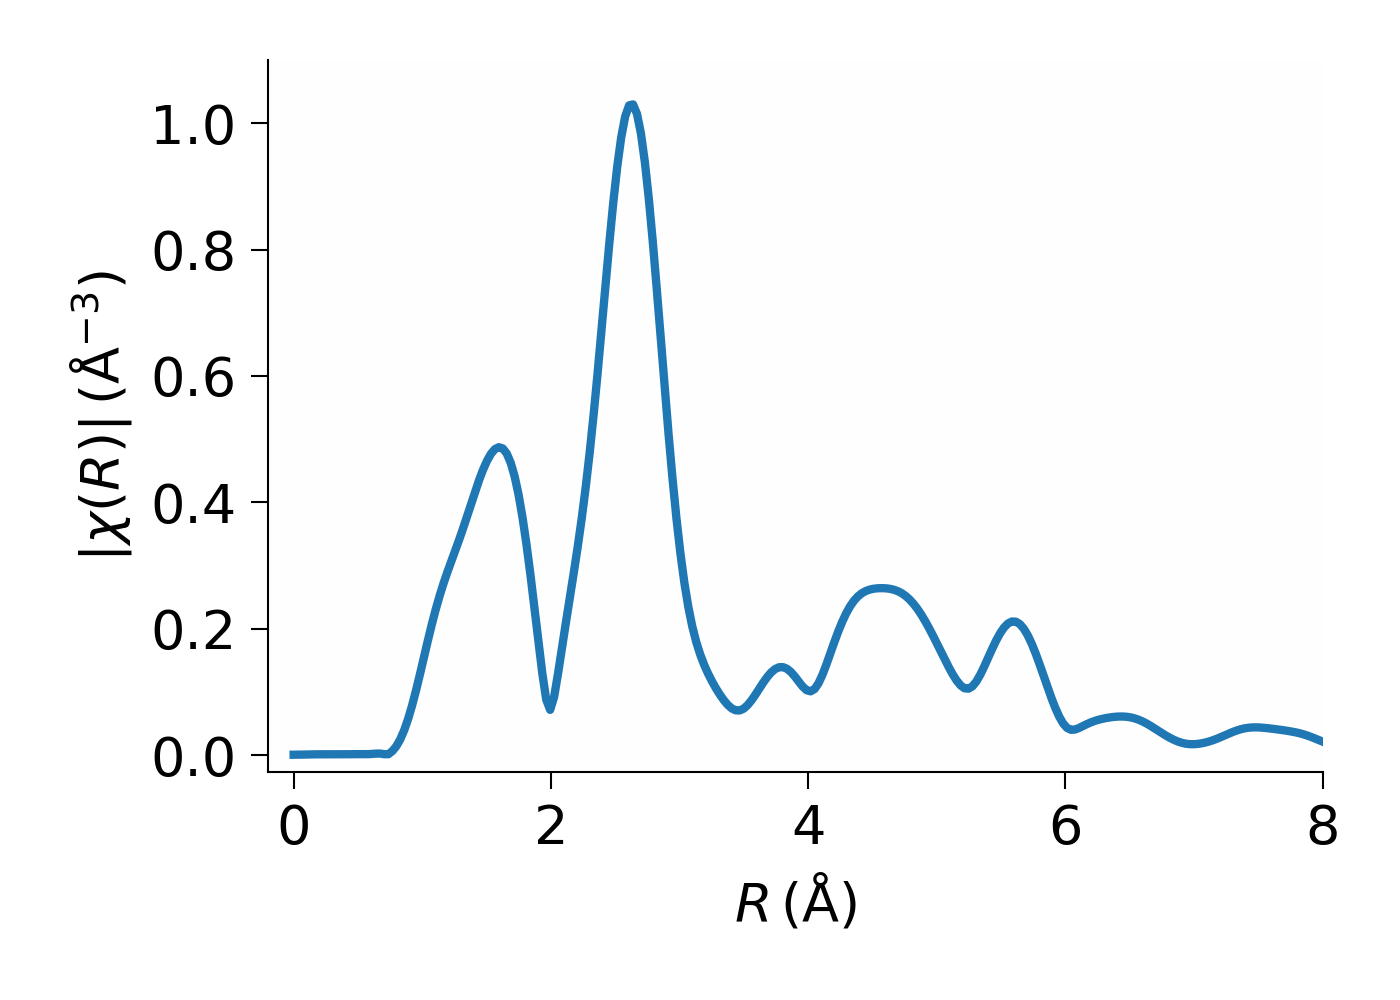
\includegraphics[width=60mm]{figs/experiment/chir}  \end{minipage}
    &
    \begin{minipage}{50mm}  \setlength{\baselineskip}{10pt}
      \hspace{-3mm}{\Red{$\chi(R)$}}

      \vspace{0.5mm}


      Peaks in {\chir} often correspond to ``coordination shells''.
      The Fe-O distance in FeO is 2.14{\AA}  -- the  first
      peak is at 1.6{\AA}.

      \vmm
      This distance shift is due to the
      {\RedEmph{phase-shift}}: ${\sin[{2kR+ {\Red{\delta(k)}}}]}$.


    \end{minipage}\\
    \begin{minipage}{70mm}
      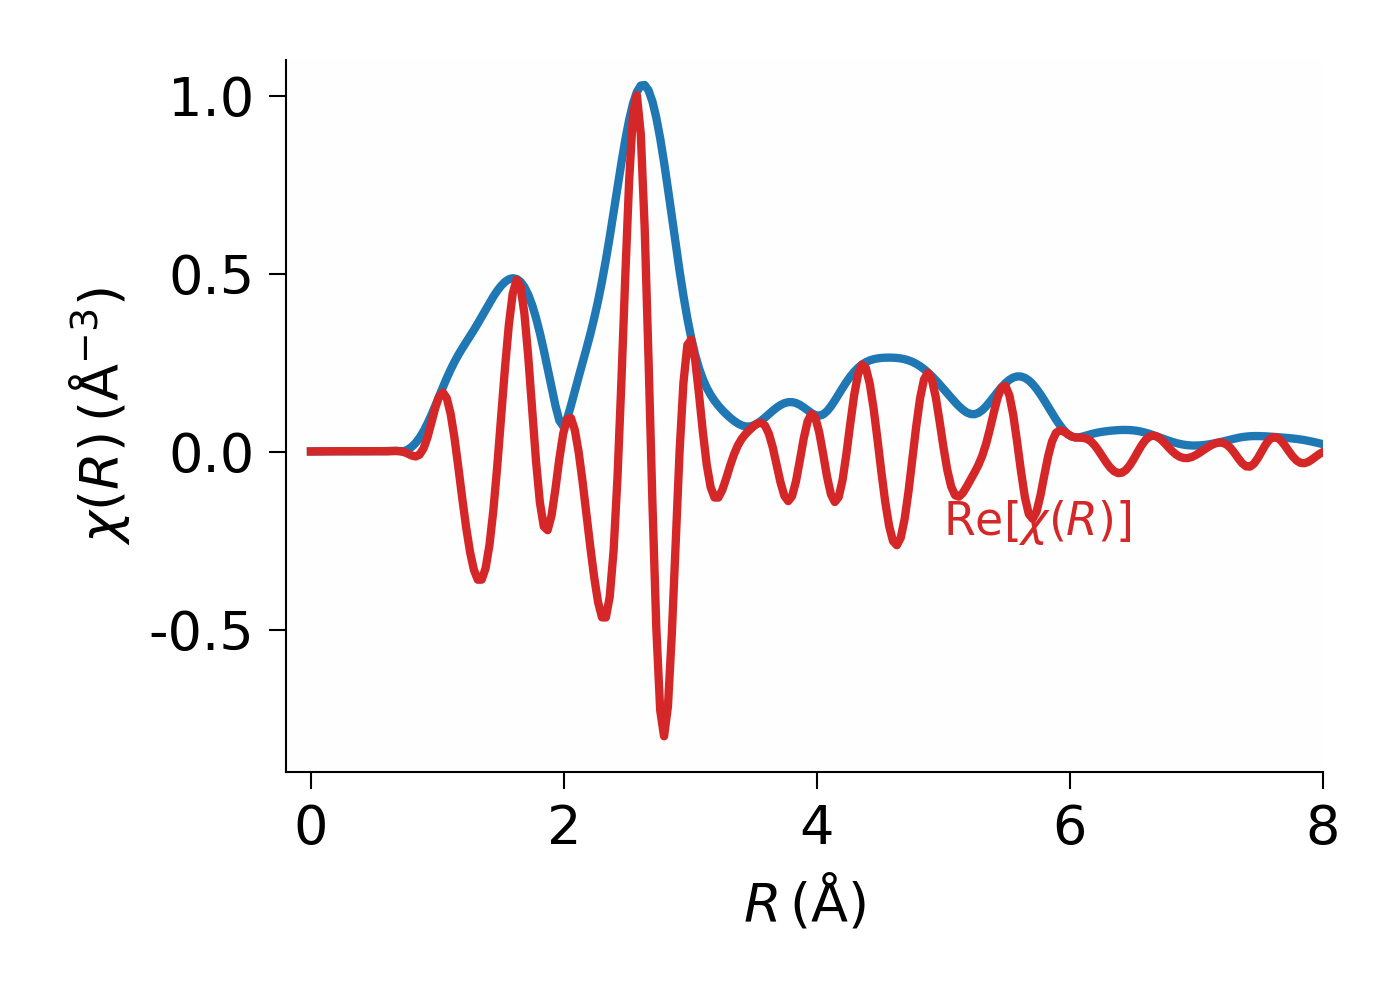
\includegraphics[width=60mm]{figs/experiment/chir_real_mag}  \end{minipage}
    &
    \begin{minipage}{50mm} \setlength{\baselineskip}{10pt}


      \vmm
      \hspace{-3mm}{\Red{$\chi(R)$ is complex:}}\vspace{0.5mm}

      Usually only the amplitude is shown, but there are
      oscillations in $\chi(R)$.

      \vmm

      Both real and imaginary parts are used in modeling.

      \vspace{3mm}
    \end{minipage}
  \end{tabular}
\end{cenpage}
\end{frame}

\begin{frame} \frametitle{Fourier Filtering}

  \begin{cenpage}{130mm}
    \begin{tabular}{ll}
      \begin{minipage}{70mm}
        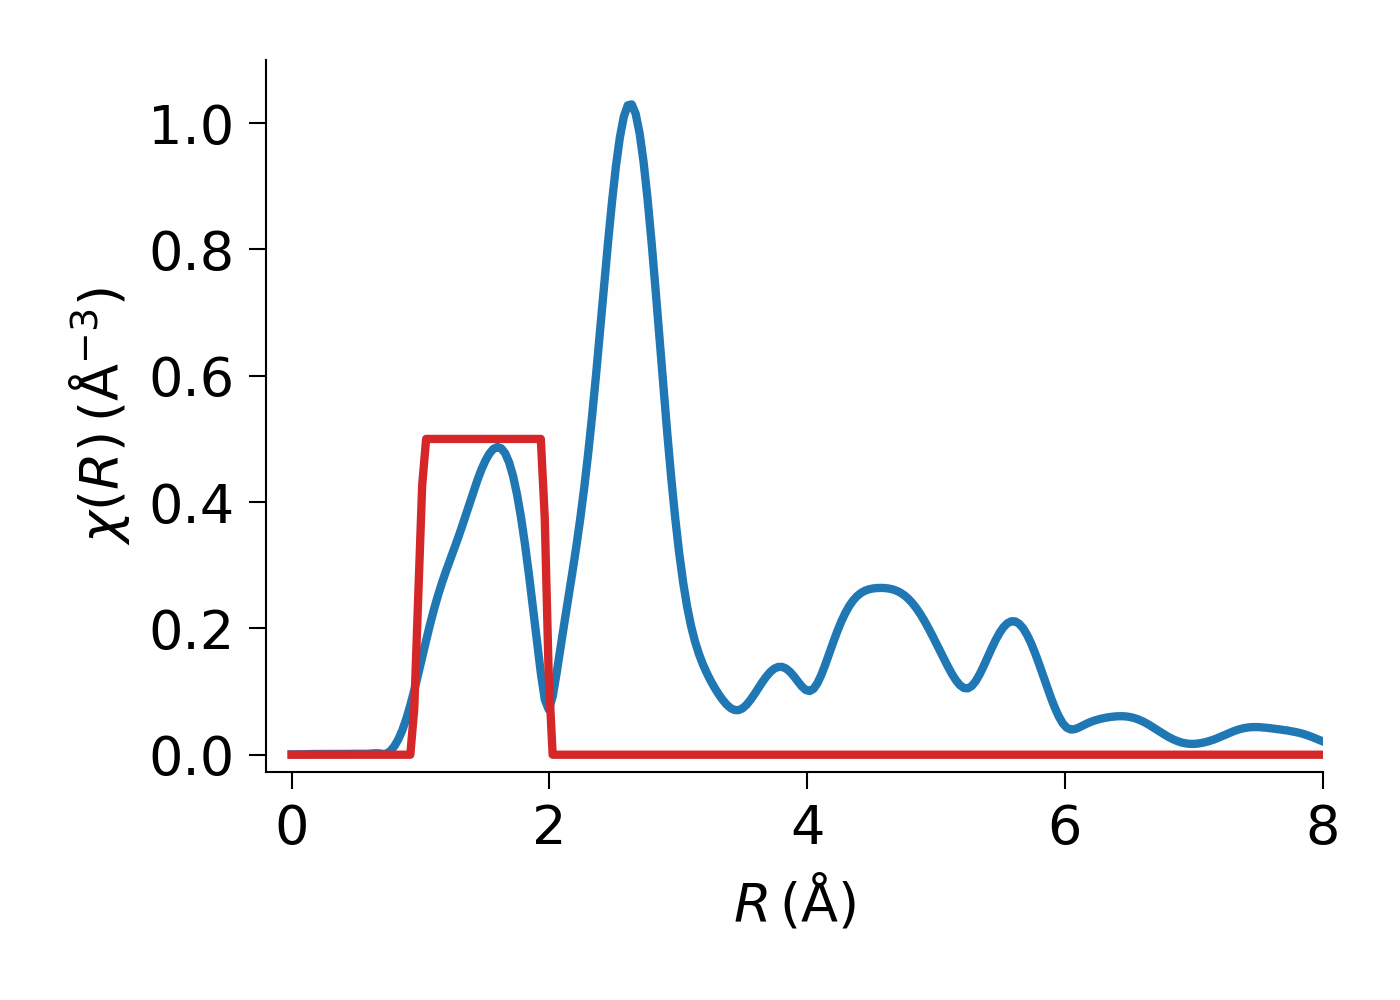
\includegraphics[width=60mm]{figs/experiment/chir_win}  \end{minipage}

    &
      \begin{minipage}{50mm}  \setlength{\baselineskip}{10pt}

        \hspace{-3mm}{\Red{$\chi(R)$}}

        often has well-separated peaks for different
        ``shells''. \vmm

      This shell can be isolated by a Filtered Back-Fourier Transform,
      using the window shown for the first shell of FeO.
       \vspace{1mm}

     \end{minipage}\\
      \begin{minipage}{70mm}
        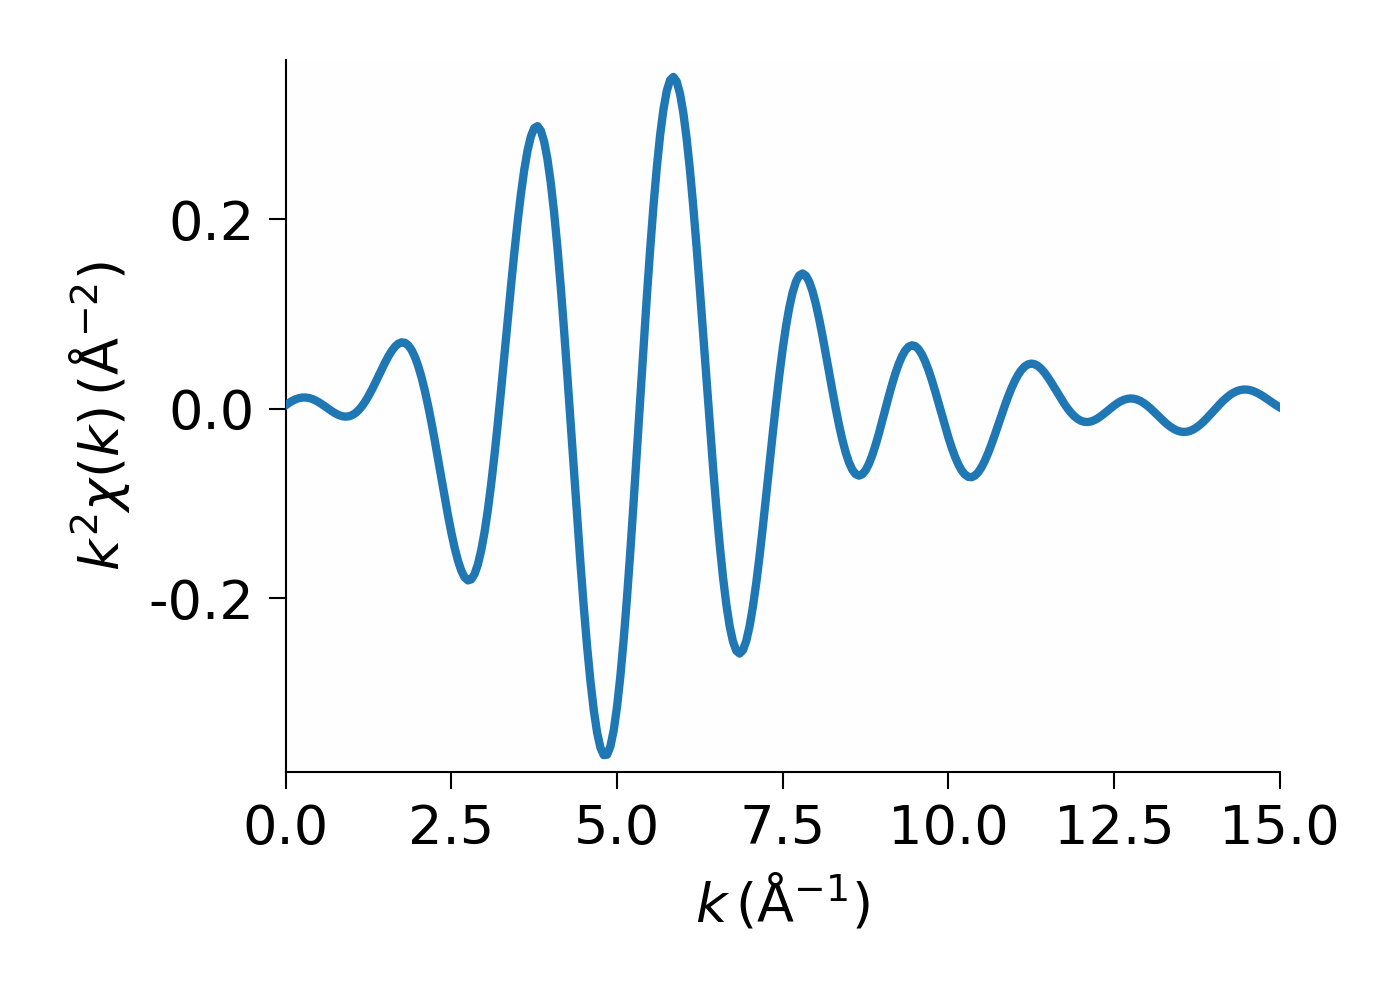
\includegraphics[width=60mm]{figs/experiment/chiq}  \end{minipage}
    &
    \begin{minipage}{50mm} \setlength{\baselineskip}{10pt}
      \hspace{-3mm}{\Red{$\chi(q)$}}  (``$Q$-space'')

      \vspace{0.5mm}

      This results in the filtered $\chi(k)$ for the selected
      shell.

      \vmm

      Many analysis programs use such filtering to remove shells at higher
      $R$.

      \vmm
      Don't do it -- it's too hard.
      \vspace{3mm}
    \end{minipage}
  \end{tabular}
\end{cenpage}

\end{frame}

\begin{frame} \frametitle{Upcoming Topics on Data Reduction and Analysis}

Now that we've seen the basic procedures, a bit more detail on these topics
is needed:

\vmm \vmm \vmm


\begin{tabular}{ll}
%%  {\Red{XANES Analysis}} & What do we do with Normalized $\mu(E)$? \\
  {\Red{Background Subtraction}} & Details on getting from $\mu(E)$ to $\chi(k)$ \\
  {\Red{Fourier Transforms}} &  Details on getting from $\chi(k)$ to $\chi(R)$ \\
  \noalign{\bigskip}
  {\Red{EXAFS Analysis}}   & Modeling to fit experimental $\chi(k)$. \\
\end{tabular}



\vfill
\end{frame}
